\section{Visualizations}\label{sec::visualizations}
\subsection{Introduction}
The last chapter introduced the first part of our Visual Analytics pipeline, the diff-algorithms in detail. Usually however sophisticated preprocessing-methods are needed, which are explained for a few applications in Chapter \ref{sec::applications}.

This chapter describes several visualizations which help analysts to gain knowledge. First, an aggregation of the two tree-structures to compare is described. Then the visualizations are detailed. Our visualizations rely on the diff-algorithms described in Chapter \ref{sec::differences} and therefore depict the tree-edit distance, that is structural (insert/delete/move/replace) and non-structural (update) operations which transform one tree-structure into the other one. Different similarity measures are used to indicate the similarity of leaf-nodes and internal nodes either based on comparing String-values via the Levenshtein-distance or in the latter case based on overlapping subtree-structures. However the usage of similarity measures is highly modular and thus other measures might be included in the future which either can be switched by user interaction or through heuristics. After briefly describing the \emph{TreeView}, the \emph{TextView} and the \emph{SunburstView} as well as basics of our specialized Sunburst layout, an explanation of filtering technique follows which together with the ID-based diffing-algorithm \footnote{usually the hash-based version comparing the hash-values of the nodes first} facilitates the analysis of large tree-structures ranging from about 100MB to even GBs of data. The key assumption underlying this efficient diff-algorithm/visualization is that similar trees are compared and therefore only a small fraction of a tree-structure has to be transformed to derive the other tree-sturcture. Querying capabilities, similarity measures and the visualization of moves are described subsequently. Next, small multiple display variants are detailed which facilitate the comparison of several tree-structures. An asymptotic runtime- and space-analysis as well as a short performance study follow. The chapter concludes with a summary.

%\subsection{GUI}
%First, a GUI framework has been developed which incorporates several views. The framework has been written from scratch based on some key-ideas and software patterns used by BaseX \cite{BASEX}. The GUI is designed to be easily extendable. It currently offers the ability to view and interact with the stored Treetank data in many ways. Incorporated are several different views. Most of them are developed to support the analysis of differences as well as similarities between tree-structures. Others will be extended in the future. Furthermore the views are synchronized meaning that several types of actions in one view are reflected in other views as well. Special care is taken to adhere to the Model View Controller (MVC) architecture with a controller managing the interactions between the views which is depicted in Fig. \ref{fig:mvc}. The next section describes the visualizations in detail.

%\begin{figure}[tb]
%\center{\includegraphics[width=\textwidth]
%{figures/mvc}}
%\caption{\label{fig:mvc} MVC-paradigm use. The \emph{TextView} and the \emph{TreeView} use standard Swing components. A \texttt{JTree} Swing-component is used implement the tree-model in the \emph{TreeView}. A \texttt{JTreeCellRenderer} implements the view and controller. It is responsible to translate user actions and to render the cells appropriately. The \texttt{JTextEditPane}-Swing component represents both the view and controller in the \emph{TextView} whereas a new \texttt{StAXDiffSerializer} described later on implements the \texttt{XMLEventReader} StAX interface to support a pull based API. It is thus the model which interacts with Treetank through a open database handle.}\end{figure} 

\subsection{Aggregation}\label{subsec::aggregation}
An aggretion of two tree-structures is illustrated in Fig. \ref{fig:aggregation}. The top half depicts the two tree-structures (revision 1 and revision 2) to compare whereas the bottom displays the aggregation or fusion of the trees based on diff-tuples observed from our ID-based diffing-algorithm. The two trees are input to the ID-based diff-algorithm which in turn fires diff-tuples. These tuples form the basis of the agglomerated tree-structure. A straight forward approach which we followed is to store the tuples in a simple List datastructure \footnote{in our case a Map which is used like a List to exchange a Java core collection map implementation with a persistent BerkeleyDB map implementation}. The colors of the nodes in the agglomeration denote if and what change is made. Deletions for instance are marked in red, whereas insertions are colored blue. Updates are not only supported for leaf nodes, as in the ContrastTreemap approach described in Chapter \ref{sec::relwork} but also for internal nodes. Furthermore the replace-operation as well as moves are supported. %Move operations are plotted via curves using hierarchical edge bundles which are drawn on top of the Sunburst layout, whereas an item indicating the position in the old tree-structure (\texttt{DiffType.MOVEDFROM}) and another item denoting the position in the other tree-structure (\texttt{DiffType.MOVEDTO}) is depicted. Items which represent updated nodes include both the value from the first tree and the value from the second tree.

\begin{figure}[tb]
\center{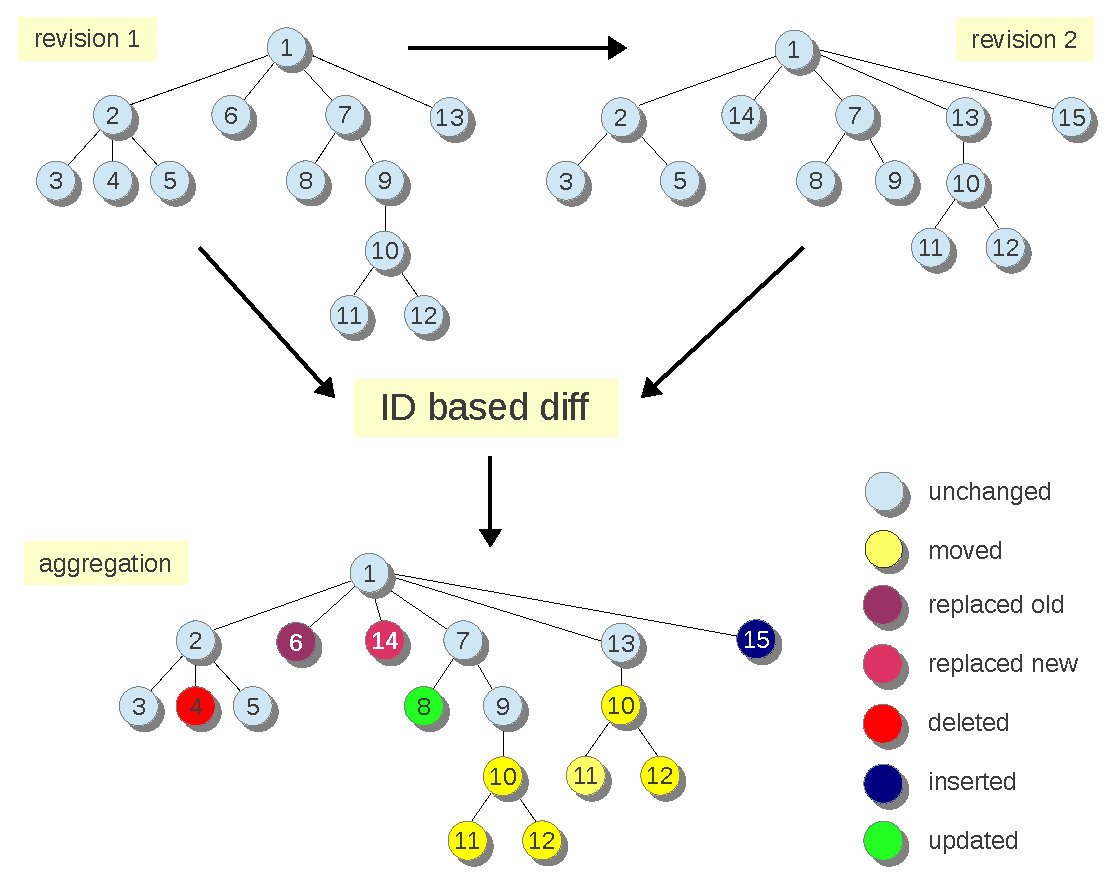
\includegraphics[width=\textwidth]
{figures/aggregation}}
\caption{\label{fig:aggregation} Two tree-structures aggregated. The numbers denote unique node-IDs. Both revisions are input to the ID-based diff-algorithm. The output represents diff-tuples including the node-IDs from both nodes which are compared in each step, the type of diff and the depths of both nodes. Storing the observed diff-tuples in an ordered data-structure forms a simple tree-aggregation.}
\end{figure} 

\subsection{Visualizations}
As described in the motivation humans are best in interpreting visual content. Therefore visualizations are developed which facilitate humans in gaining new insights and quickly detecting differences in tree-structures. Next, all available views are described in detail. %An XML based serializ   ation view of the tree-structure   %A few of them currently only support the visualization of one revision of the tree-structure. While not being of exceptional value for comparing trees besides viewing two instances of the GUI side by side they will most probably be extended to support

\begin{itemize}
\item
First, a \emph{TreeView} displays nodes in a tree structure just like visual frontends for filesystems as illustrated on the left side in Fig. \ref{fig:treetextview}. Nodes either can be expanded to show all child nodes which are inside the current viewport or collapsed to hide children. The subtree of a selected node is marked with a background color. Currently the view is not able to incorporate the aggregation and thus is not further described.

\begin{figure}[tb]
\center{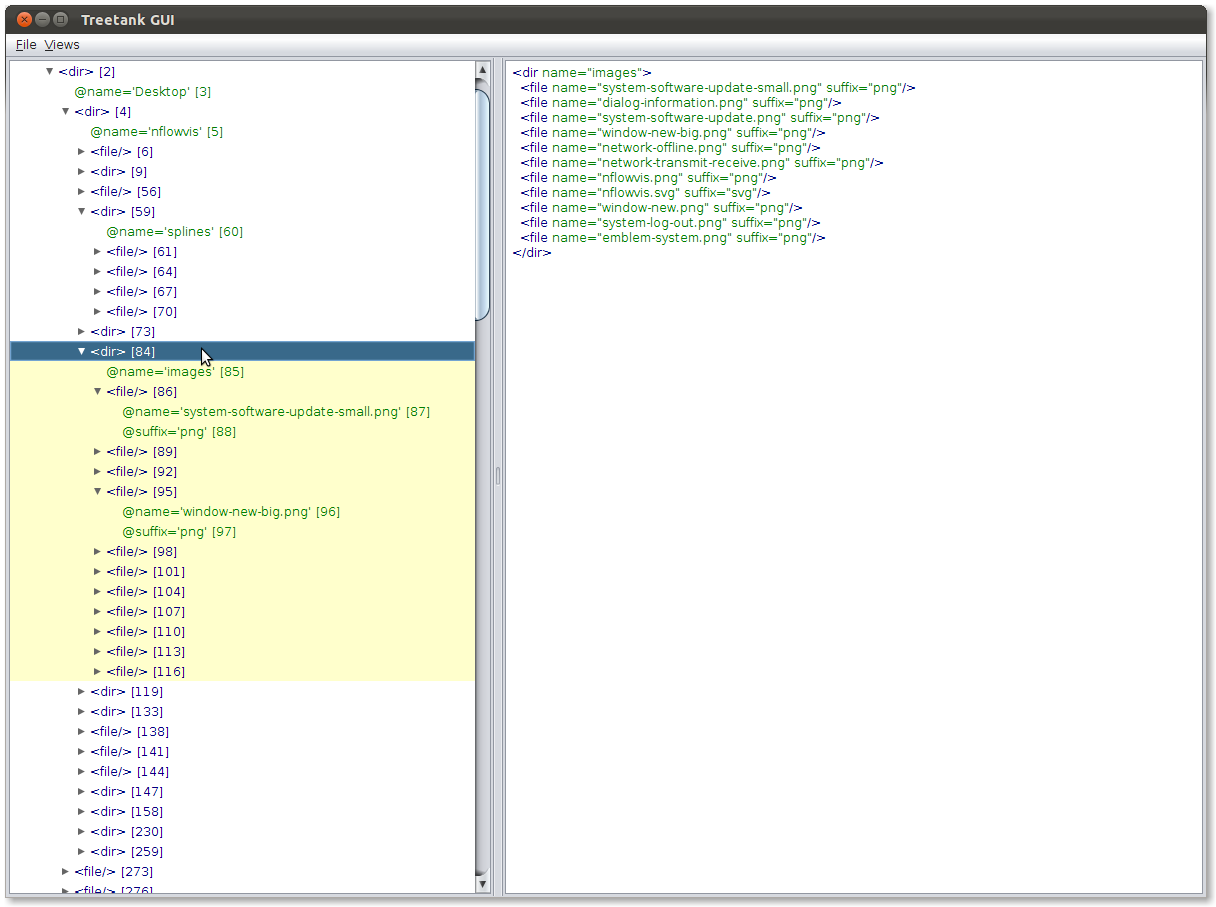
\includegraphics[width=\textwidth]
{figures/treetext}}
\caption{\label{fig:treetextview} TreeView and TextView side-by-side}
\end{figure}

\item
The \emph{TextView} displays serialized XML-documents or fragments and supports syntax highlighting. Moreover it just serializes the part of data which is currently viewable and an additional small overhead of pixels to enable scrolling. Other data is serialized and appended while scrolling down. A reusable pull-based StAX-parser supports the syntax highlighting, serialization of end-tags as well as the append-approach.%A new \emph{StAX}-parser implementation provides a pull-based API to support this "append-on-scroll" behaviour. It provides two features. Since it is pull based the application (the GUI) can determine when and how much data is parsed. Furthermore it provides the parsed node kinds which are used to support syntax highlighting. Simply using a \texttt{DescendantAxis} from Treetank which traverses the nodes in preorder is not sufficient. End-tags have to be emitted as well. Therefore we opted for developing a reusable \texttt{StAX}-implementation. Nontheless the \texttt{DescendantAxis} is used internally as part of the implementation to traverse the tree in preorder. To adhere to the specifications of the methods which must be implemented and to keep the iterator-methods idempotent is the biggest challenge. In addition to generate events for end-tags the StAX-parser supports a \texttt{peek()}-method to receive the next event without moving forward.

Fig. \ref{fig:treetextview} displays the \emph{TreeView} and the \emph{TextView} side by side. Note that the two views are kept in synchronization.

\begin{figure}[tb]
\center{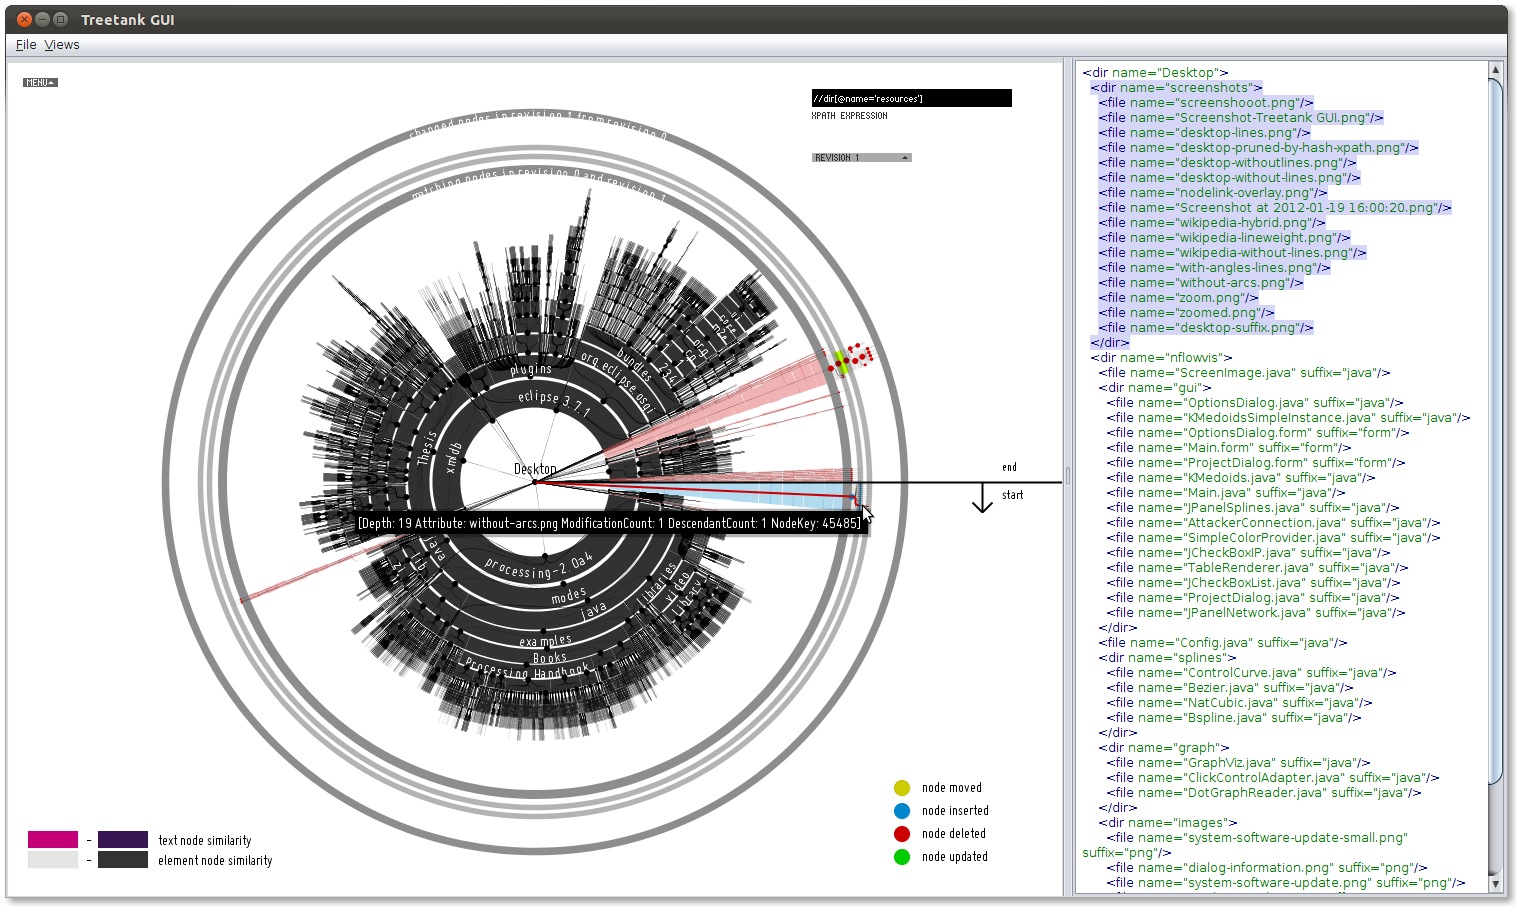
\includegraphics[width=\textwidth]
{figures/sunbursttextview-overview}}
\caption{\label{fig:sunbursttextview} SunburstView and TextView side-by-side.}
\end{figure}

In order to support an analyst with the task of analysing differences in tree-structures the view supports another mode which incorporates the aggregation of the two tree-structures to compare described in section \ref{subsec::aggregation}. Based on this aggregation a second pull-based parser is developed. The depths of the diff-tuples in the aggregated structure are used to determine when to emit end-tags. A dedicated background-color is used to mark the type of diff. In case an updated node is encountered the old value and the new value is emitted. The view in contrast to the \emph{SunburstView} which is described next is not able to visualize connections between the old and new location of moved nodes. %It receives a \texttt{DiffAxis} to iterate over \texttt{SunburstItem}s created for the \emph{SunburstView} which is described next. We support a preorder-traversal of the items to derive the stored diff-types as well as the depths in the items. The depth of the current item and the depth of the next item using a \emph{peek()} method on the \texttt{DiffAxis} are used to determine if an end-tag must be emitted. Another check involves empty-Elements whereas an \texttt{EndElement} must be emitted immediately following the \texttt{StartElement} in for the next call to \texttt{nextEvent()}. In this case the parent node-IDs must match. Furthermore the depths are used in subsequent calls to \emph{nextEvent()} to determine how many closing tags must be emitted. In case of \texttt{ElementNode} updates we immediately emit the new updated element and push the old element on an end-tag stack. In a subsequent call to \texttt{nextEvent()} the old value in case of a \texttt{TextNode} or the old element in case of an \texttt{ElementNode} are emitted. Changed nodes are highlighted with a background color which denotes the kind of change. The \texttt{TextView} itself must not change the indentation for the old value/old element if an \texttt{UPDATE} is detected. Only the first emitted value (the new value) must change the indentation. 

A legend which describes the color $\leftrightarrow$ change mapping is currently only available from within the \emph{SunburstView}. However this is only an implementation detail and a help-dialog will be added in future releases. Exemplary a side-by-side view with the \emph{SunburstView} is depicted in Fig. \ref{fig:sunbursttextview} whereas the first inserted subtree is also visible in the \emph{TextView} area, marked by a blue background-color. 

While the \emph{SunburstView} as we will shortly see provides a great overview about the whole tree-structure and subtrees, the \emph{TextView} provides a better detailed view on selected subtrees. Other deficiencies meantioned in the introduction regarding the boundary of nodes and XML-specific details do not apply as we compare the tree-structure with the ID-based diffing-algorithm in the first place instead of comparing single characters line by line. Besides the lack of an appropriate overview, which is one of the advantages of the \emph{SunburstView}, the \emph{TextView} is an ideal partner to the \emph{SunburstView} as the XML text-serialization is better readable than radial Sunburst labels.

The diff-algorithm is only ever called once for every visible view\footnote{the only exception are small multiple displays which represents changes among several tree-structures}. The diff-tuples are then broadcasted to all other views which are capable of displaying the aggregated tree-structure.

\item
The \emph{SunburstView} displays a tree structure in a radial layout (Fig. \ref{fig:sunburstview}). We first describe the basics to display one tree-structure and extend the approach to include the aggregated tree-structure to display the differences between two tree-structures. The Sunburst-layout is a space filling approach, thus aiming for a maximized usage of available screen space for the hierarchical visualization. Furthermore it is an adjacency based approach, drawing child nodes next to their parent node. In contrast, Treemaps enclose child-nodes within parent nodes. Thus a Treemap utilizes available screen space to the full extend as the root node occupies the whole available screen space recursively embedding descendants as rectangles. In contrast, in the Sunburst method corners are left empty due to the radial representation. While this alone on first glance might be a great drawback in addition to circular segments which are more difficult to read regarding node labels and comparisons of item-sizes, the layout is stable even if a lot of changes have to be displayed and the hierarchical structure is much better readable. The Spiral Treemap layout which has been described in Chapter \ref{sec::relwork} is relatively stable but it is still very difficult to track changes which might be scattered through 90° degree changes in direction as well as the complicacy to follow nested rectangles which are arranged in spirals in comparison to the simplicity of a Sunburst layout.

The root node of a tree-structure in a Sunburst-layout is plotted in the middle of the screen depicted as a circle. Child-nodes of the root node are drawn in circular segments next to their parent. The radius depends on the depth. It shrinks with increasing depth such that the area of circular-segments between two levels does not change. Otherwise items toward the edges occupy more space. However this behaviour can be changed to further visually emphasize changes which will be visualized along the edges (section \ref{subsec::comparison}). The arc of an item, which depicts one node, in the Sunburst layout depends on one or more node-attributes. A relative measure in regard to the other children is used.

\begin{figure}[tb]
\center{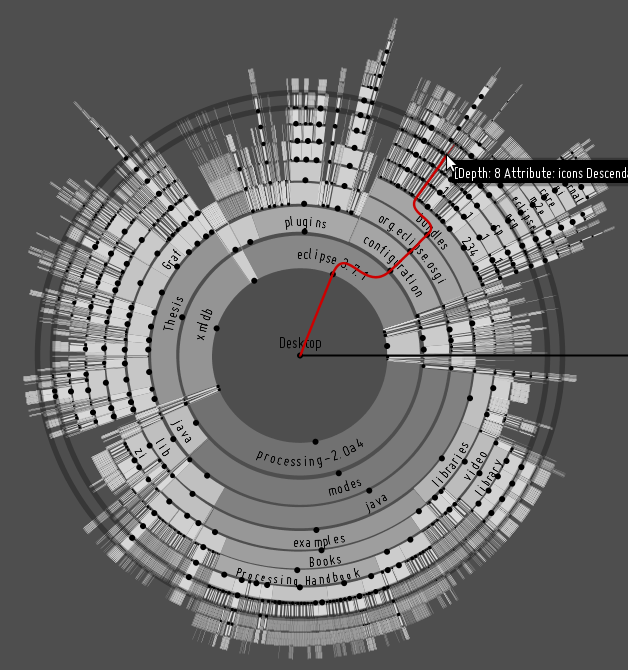
\includegraphics[width=\textwidth - 7em]
{figures/sunburstview-cut}}
\caption{\label{fig:sunburstview} SunburstView depicting the structure of the authors filesystem directory ``/home/johannes/Desktop''.}
\end{figure}

In our case the subtree-sizes are mapped onto the extend of each item such that nodes having more descendants occupy more space. The formular is straight forward:

\begin{equation}
extend = \left\{ \begin{array}{cl}
2 \cdot \pi & \textrm{if }node\ is\ root\ node\\
parentExtend \cdot descs / (parentDescs - 1) & \textrm{otherwise}\end{array}\right.
\end{equation}

Note that we recently added the number of descendants of each structural node in Treetank to maximally speed up the creation of the visualization. 

The color of each item in case of internal nodes (element nodes) is mapped to the subtree-size of a node. \texttt{TextNode}s are colored according to their text-length.

A node-link diagram is drawn on top of the \emph{SunburstView} to further emphasize the hierarchical structure. Dots representing the node in addition to the SunburstItem-segment are depicted in the center of the item whereas either bezier curves or straight lines denote a child/parent-relationship between the nodes.

In order to support large tree-structures the generated Sunburst-items are drawn into an offscreen buffer, whereas the items are only used to implement a mouseover effect and to support XPath-queries with subsequent highlighting of the resulting nodes/items.

\subsubsection{Interaction}
The view is highly customizable. Checkboxes enable or disable plotting the node-link overlay and/or the Sunburst-arcs to either emphasize the parent/child relationship or subtree-sizes\footnote{subtree-similarities in the comparison mode}. Furthermore the line/curve-thickness denoting parent/child relationships and the dot-sizes are adjustable.

%\begin{figure}[tb]
%\center{\includegraphics[width=\textwidth]
%{figures/sunburst-adjusted-scale-cut}}
%\caption{\label{fig:sunburst-adjusted-scale} SunburstView - adjusted arcs/dotsize parameters}
%\end{figure}

%Figure \ref{fig:nodelink} illustrates the node-link overlay without coloring the arcs. The red curve marks a path up to the root-node through all ancestor-nodes for the current node which is highlighted by moving the mouse over the item.

%\begin{figure}[tb]
%\center{\includegraphics[width=\textwidth]
%{figures/nodelink}}
%\caption{\label{fig:nodelink} node-link diagram}
%\end{figure}

To support different mappings from node-attributes to the color of Sunburst-items, a term which is used interchangeably in the following sections, a linear-, squareroot- and logarithmic-normalization is available.

Crucial to the interaction and the value of the visualization itself is the possibility to drill down into the tree. Clicking an item results in drawing the selected node with its subtree in a new Sunburst-diagram whereas the selected node becomes the new root. Furthermore a simple, fast undo-operation is supported as we keep track of offscreen-buffers and the items. %Stacks are used to implement a simple undo-operation which is very fast as we store the Sunburst-items as well as the background buffer-image. 

A well known technique to enlarge small regions is to use transformations of the screen-space, as for instance a fisheye lense to select very tiny items. The enlargement of small items via a fisheye lense is depicted in Fig. \ref{fig:fisheye}. Zooming and panning is also incorporated allowing affine transformations of the screen (Fig. \ref{fig:zoom}) to analyse important regions. Note that the mouseover-effect displaying additional information about the node itself as well as the legends are not affected by the transformation. As the background-buffer cannot be used in this case zooming is restricted to smaller trees with an upper bound of about 10\_000 to 15\_000 nodes.

\begin{figure}
\centering
\subfigure[Fisheye transformation]{
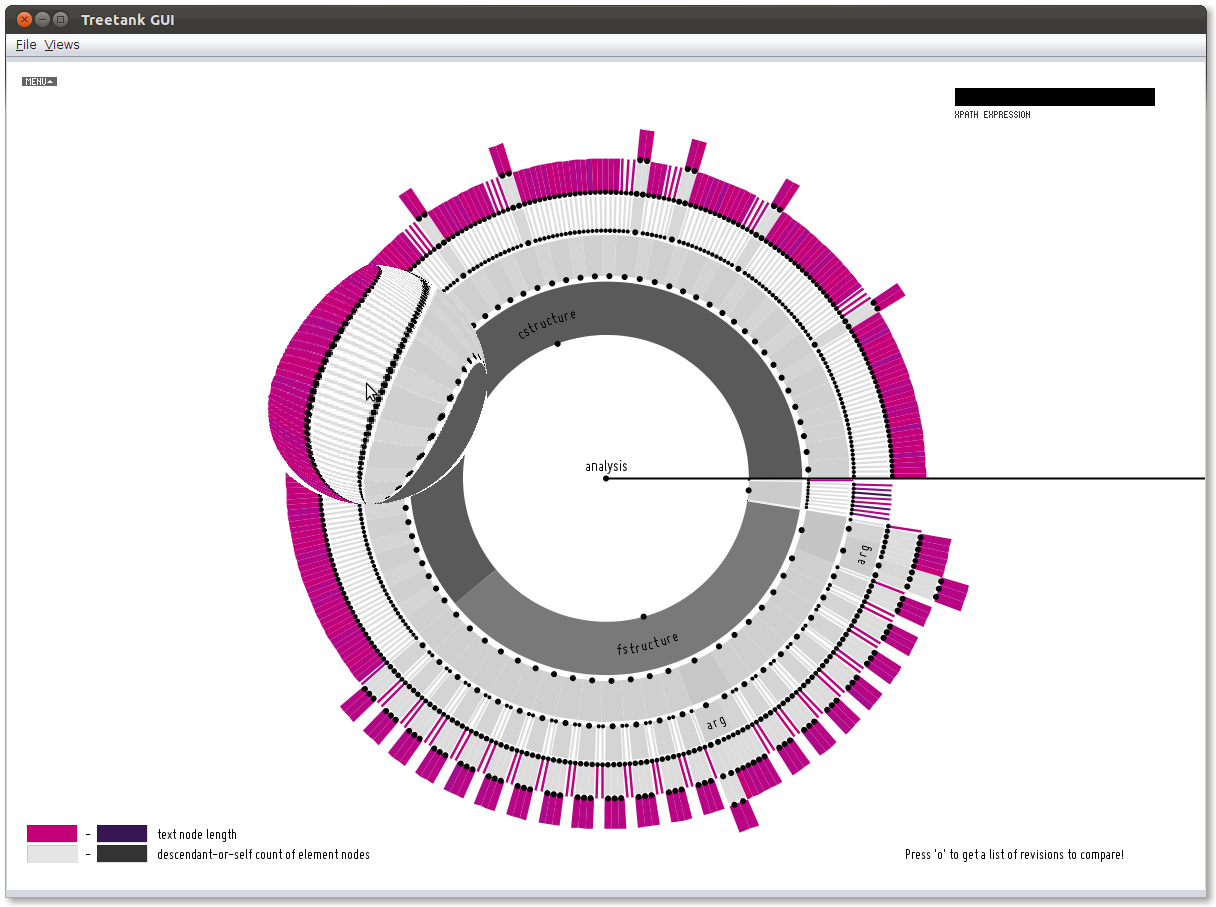
\includegraphics[width=\textwidth - 3em]
{figures/fisheye}
\label{fig:fisheye}
}
\subfigure[Zooming into the visualization]{
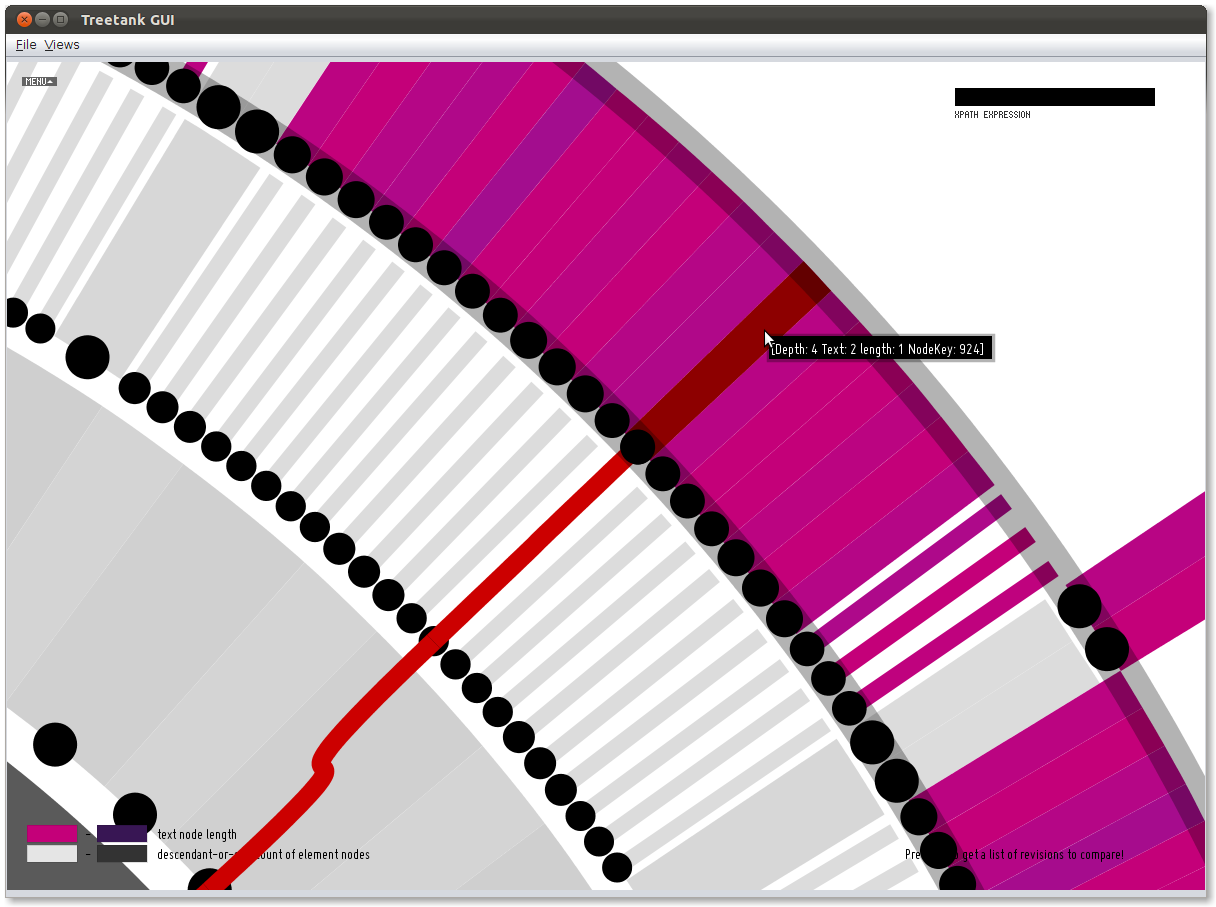
\includegraphics[width=\textwidth - 3em]
{figures/zooming}
\label{fig:zoom}
}
\caption{Techniques to enlarge regions of interest.}
\end{figure}

In order to manipulate Treetank resources it is even possible to insert XML fragments as right-siblings or first-childs as well as to delete nodes.

\subsubsection{Querying}
XPath is usable to query the tree-structure for specific nodes. Result sequences are highlighted in a light green. Fig. \ref{fig:sunburstxpath} displays the result of a simple \texttt{//*[text()='var:0']} query to highlight all nodes which have a text-node child with the value ``var:0''.

\begin{figure}[tb]
\center{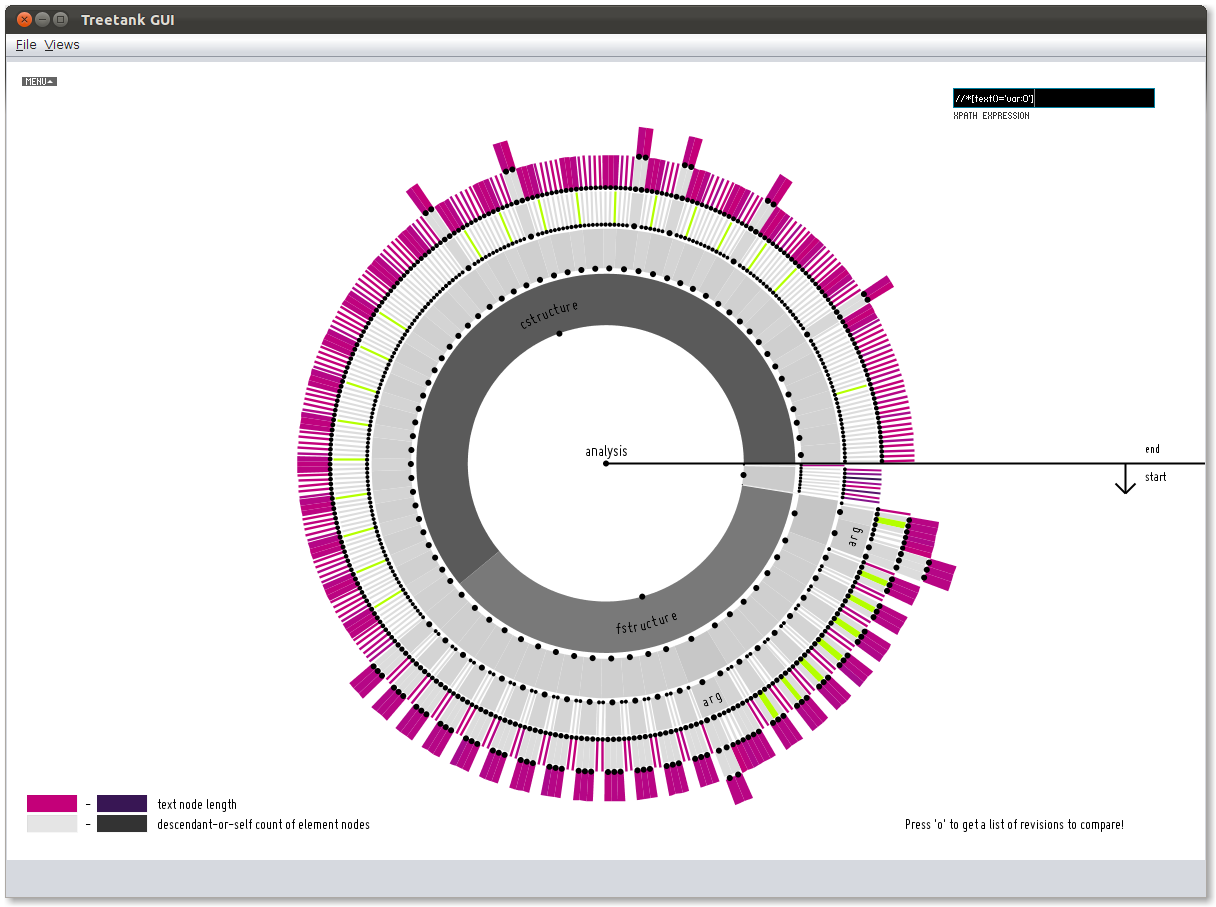
\includegraphics[width=\textwidth]
{figures/sunburstxpathquery}}
\caption{\label{fig:sunburstxpath} XPath query results displayed in light green}
\end{figure}

\subsubsection{Labels}
Whenever the Sunburst items sufficiently large and an adaptable scale to draw the arcs for each depth is greater than a predefined value, labels are drawn. Labels in the top half of the visualization, that is if the center of the item is greater than $\pi$, are drawn beginning at the start-angle in clockwise direction, otherwise they are drawn starting from the end-angle in counter clockwise direction. Furthermore the font-size is limited to a range between two values, whereas the size is decreased with an increased depth. 

\subsubsection{Filtering/Pruning}
The standard \emph{SunburstView} optionally filters the tree by level. While this filtering is not perfect in circumstances where the fanout is very large, it works very well to keep the number of generated Sunburst items small. Furthermore the view currently is used as an entry point to the comparsion view which is also based on the Sunburst-layout whereas it is planned to backport the filtering by itemsize.

Whereas it is sufficient to use an XPath-query as for instance \\
\texttt{//*[count(ancestor::*)<3]} to get a sequence including all nodes between level 0 and 3 we opted for a tree-traversal implementation, as the XPath query has to touch all ancestor nodes in the current Treetank implementation due to our encoding which does not utilize hierarchical node-IDs as for instance the ORDPATH/Dewey-IDs where it is usually trivial to compute such queries on the ID itself in an in-memory B*-tree or another datastructure.
\end{itemize}

\subsection{Comparsion using a new Sunburst-layout algorithm}\label{subsec::comparison}
The standard \emph{SunburstView} includes a comparison-mode. Once a base revision is opened and the \emph{SunburtView} is enabled an analyst is able to choose another revision from a dropdown menu for comparison. Note that all interaction capabilities described earlier are also available in the comparison mode. Differences and additional capabilities are described in the following sections. In order to compare tree-structures in a radial arrangement similar to the described SunburstView which facilitates exploring a single revision a new layout-algorithm is developed. Next, we first describe the new layout.

\subsubsection{Sunburst Comparsion-Layout}
The Sunburst comparison layout is illustrated in Fig. \ref{fig:sunburst}. Nodes are colored as depicted in the color legend in the bottom right corner. All nodes which are unchanged during the comparison of revision 0 and 1 are plotted inside the inner circle which is labeled ``matching nodes in revision 0 and revision 1''. The circle itself is drawn between the maximum level of the unchanged nodes plus one and maximum level plus two. Changed nodes are zoomed out from their original place and drawn between the two dark circles labeled ``changed nodes in revision 0 and revision 1'' and ``matching nodes between revision 0 and 1''. Fig. \ref{fig:sunburst} depicts the area with hatches. Similarly the arrows emphasize the direction in which changed subtrees are zoomed/dislocated. Both, the hatches and the arrows are only drawn to stress our design decisions and the semantic zoom which serves a double purpose. First, the visualization adheres to a Tree-Ring metapher depicting the evolution of a tree. Just like the age of a tree in the nature is deducable by analysing rings in a cross-cut of the stem whereas the rings denote the age and each ring represents one year starting from the center to the outside, our prototype aims at representing the changes between two rings. In our visulization the unchanged nodes form the center of the \emph{SunburstView} whereby changed nodes are zoomed to the border between the inner and outer ring which is representing the growth of a tree in case of analysing temporal tree-structures. Additionally, this transformation displaces changed subtrees to a prominent place. Thus, small changed subtrees or even single node-changes are much better noticeable as they are not surrounded by unchanged subtrees which might even be deeper. To depict changes between multiple trees or several revisions of a tree first considerations involved the addition of changes from a sequence of sorted revisions in further rings. The center thus represents unchanged nodes between \emph{all} compared revisions whereas changes between selected or consecutive revisions are drawn between new appended rings. According to the Tree-Ring metapher each comparison between a pair of trees appends a new ring denoting the changes. Therefore two rings denote the boundaries between the changes of comparing two revisions. However, this affects the whole layout each time. The idea proved to be not viable because of complexity issues. To name a few

\begin{figure}[tb]
\center{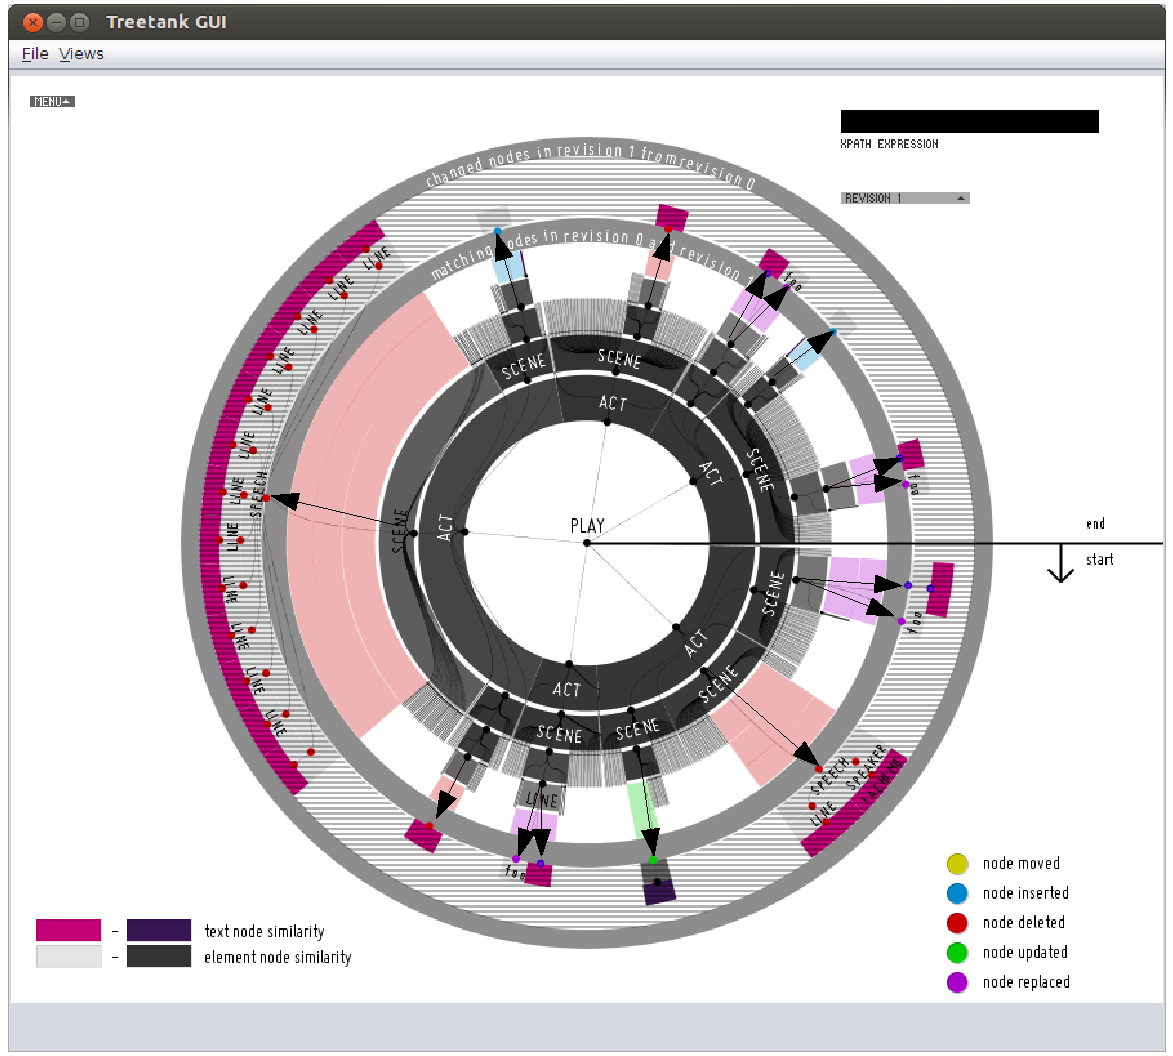
\includegraphics[width=\textwidth]
{figures/sunburst.pdf}}
\caption{\label{fig:sunburst} SunburstView - comparison mode.}
\end{figure}

\begin{itemize}
\item The center must keep space between unchanged nodes/subtrees for all upcoming changes (between all compared trees/revisions).
\item Consecutive calling the diff-algorithm and merging diffs into a single aggregated tree-structure.
\item Keeping track of all opened transactions on each revision and resetting the transaction appropriately depending on the revision in which a change has occured to derive node-labels.
\item Similarly the depth for items in the tree will change very often which involves further state and it is almost not possible to denote the current depth during a preorder traversal of the aggregated tree-structure (depending on the tree-structure itself).
\item The \texttt{subtree-size} and \texttt{modification}-count of each nodes' subtree will be cumbersome to calculate.
\end{itemize}

These and similar complexity considerations formed the idea of introducing small multiple displays instead, which are described in section \ref{subsec::smallmultiple}.

\subsubsection{Short animation}
In order to clearly demonstrate the semantic zoom which dislocates items a short animation is implemented as test persons usually do not grasp the meaning without further explanation. Thus the transformation of changed subtrees is shown which dislocates the items to their dedicated positions along the arrows in Fig. \ref{fig:sunburst} \footnote{remember, the arrows are not drawn in the visualization, they are just added to the screenshot to emphasize the transformation}. However the animation depends on the number of Sunburst items which are created and thus is skipped depending on a threshold to avoid a reduction of the framerate (frames per second). Similarly zooming/panning is not allowed if too many items are generated.

\subsubsection{Layout algorithm}
After invoking the ID-based diffing-algorithm and collecting observed changes, the new Sunburst-layout is drawn. First of all, based on the aggregation of the compared trees, Sunburst items are created. The diff-tuple which denotes a node in the aggregation is of the following form: key in first revision / key in second revision / depth in first revision / depth in second revision / type of diff. The Sunburst items are created during a preorder traversal of the diff-tuples. Initially we developed an axis based on the key idea to traverse the tree-structure of the newer revision and change a transaction cursor to the old revision whenever a deleted, moved (the old place) or replaced (the old) node is encountered. The advantage is that node-pointers are usable as a guidance to traverse the aggregation in preorder. Note, that the tree-aggregation in contrast is based on the diff-tuples and thus does not include direct pointers to follow. Therefore we first opted for the pointer-based to follow node-pointers with a read-transaction. The current-transaction is temporally replaced by a transaction opened on the old or back to the one opened on the new revision depending on the current type of diff. However the pointer-based preorder-traversal beares a lot of complexity as the node-ID of the next node to traverse has to be set in advance and the movement of the transaction in a lot of cases cannot be immediately reflected by adjusting datastructures which are required to determine the start-angle, end-angle, subtree-size and other attributes of a Sunburst item. Fig. \ref{fig:tree-axis} demonstrates a lot of this complexity on a simple tree-aggregation. Note that the terms ``aggregation'' and ``agglomeration'' are used interchangeably in this thesis. 

\begin{figure}[tb]
\center{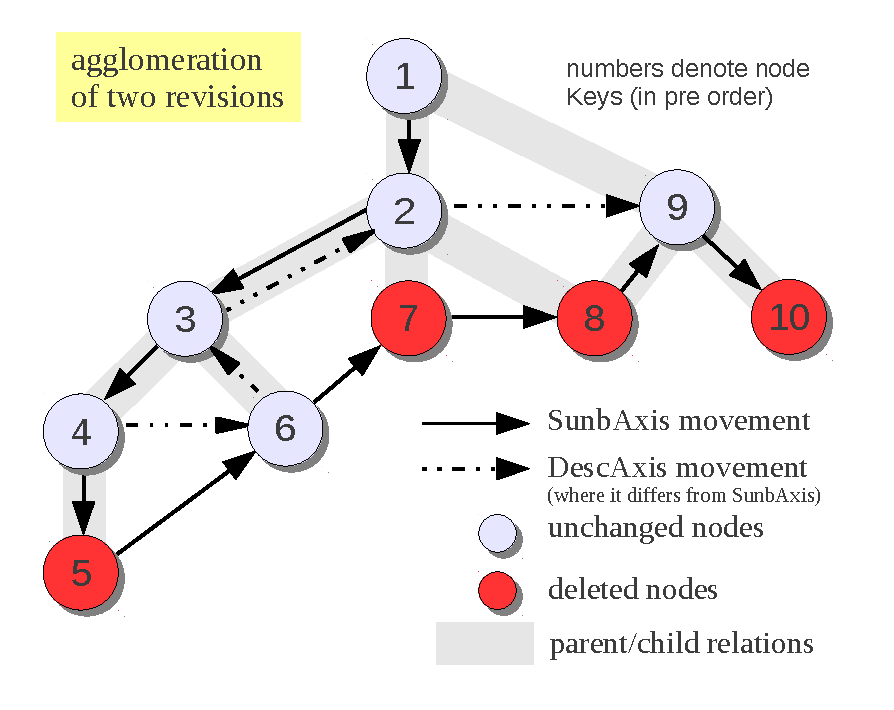
\includegraphics[width=\textwidth - 12.5em]
{figures/tree-axis}}
\caption{\label{fig:tree-axis} SunburstCompare-Axis based on node-pointers.}
\end{figure}

If the transaction is located at the node with the node-ID/nodeKey 4 the next node returned following pointers\footnote{for instance in the DescendantAxis} is the node denoted by node-ID 6 because node 5 is deleted and thus not referenced and not available in the newer revision. As such it is not sufficient to follow only child-node pointers. Thus additionally the depth of the next diff-tuple must be compared to the current depth. Furthermore the kind of movement must be tracked to adjust datastructures used to determine all Sunburst item attributes required (start-angle, end-angle, number of subtree modifications...).

Another example of the complexity is the movement from node 6 to node 9. Usually the next node will be node 9, however in our case the next node must be the deleted node 7. Thus internal stacks keeping track of attributes which are required for new sunburst items in many cases must be adapted differently than during a simple preorder traversal of a single revision.  %only one element must be removed from the stack instead of two. Each time a \texttt{DELETED} or \texttt{MOVEDFROM} diff type is encountered the transaction is temporarily changed along with the nextNodeID which denotes the ID the transaction in the $hasNext()$-method must move to the next time called and a right-sibling node stack which is used in cases where the node has no first child and no right sibling. In this case the next node-ID is removed from the right-sibling stack (a node-ID is pushed on the stack for each child-movement whenever the node (before the move to the first child has a right sibling) and the depth must be adjusted accordingly, too.

%Similarly if the movement is to the next following node (on the XPath \texttt{following::}-axis) and the next node will not be of the kind \texttt{DELETED} and \texttt{MOVEDFROM}, the actual movement cannot be done before the next call to $hasNext()$.% and the method is very similar to algorithm \ref{algo:popStacks}.

%\begin{algorithm}[Hhtbp]
%\SetAlgoLined
%\SetKwInOut{Input}{input}\SetKwInOut{Output}{output}
%\Input{int initDepth, DiffTuple diffTuple, DiffTuple lastDiffTuple, EMoved moved}
%\Output{nothing, the instance variables are directly modified (method/algorithm has side effects)}
%\BlankLine
%int tmpDepth = 0\;
%\If{mDepth == 0}{
%  tmpDepth $\leftarrow$ initDepth\;
%}\Else{
%  tmpDepth $\leftarrow$ lastDiffTuple.getDepth().getNewDepth()\;
%}
%\If{mMoved == EMoved.ANCHESTSIBL}{
%  \If{tmpDepth - initDepth $>$ diffCont.getDepth().getOldDepth() - initDepth} {
%    \tcp{Must be done on the transaction which is bound to the new revision.}
%    boolean first $\leftarrow$ true\;
%    \While{tmpDepth - initDepth $>$ diffCont.getDepth().getOldDepth() - initDepth} {
%      \If{first == true}{
%        \tcp{Do not pop from stack if it's a leaf node.}
%        first $\leftarrow$ false\;
%      }\Else{
%        mDiffStack.pop()\;
%        mAngleStack.pop()\;
%        mExtensionStack.pop()\;
%        mParentStack.pop()\;
%        mDescendantsStack.pop()\;
%      }
%
%      tmpDepth--\;
%      mDepth--\;
%    }
%  }\Else{
%    moved $\leftarrow$ EMoved.STARTRIGHTSIBL\;
%    mAngle += mExtension;
%  }
%}
%\caption{adjusting stacks and depths for movement to next following node for the first DELETED or MOVEDFROM node after another type has been encountered}\label{algo:popStacks}
%\end{algorithm}

The last pitfall in Fig. \ref{fig:tree-axis} occurs after traversing the node denoted by node-ID 9. Usually the traversal is finished but in this case the deleted node ``10'' follows.

We observe that following node-pointers to traverse the aggregation is very complex in terms of a lot of special cases have to be handled and thus is a performance issue as well due to a lot more comparsions and instructions.

The complete algorithm therefore is omitted as we developed a second, in comparsion lightweight algorithm. Instead of using a pointer based traversal it became apparent that it is easier to directly use the diff-tuple and move either the transaction opened on the old revision or the transaction on the new revision depending on the diff-type.

The outline of $hasNext()$, a method which returns \texttt{true} if the preorder traversal is not finished or \texttt{false} otherwise, is described in algorithm \ref{algo:skeleton}.

\begin{algorithm}[tb]
%\SetAlgoLined
\SetKwInOut{Input}{input}\SetKwInOut{Output}{output}
\Input{(instance variables) INodeReadTrx mOldRtx, INodeReadTrx mNewRtx, boolean mHasNext, int mDepth, int mNextDepth}
\Output{true, if more diffs are in the diff list, false if index == size}
\BlankLine
\tcp{Fail if there is no node anymore.}
\If{!mHasNext}{
  return false\;
}

\tcp{Setup everything.}
setupDiffs()\;

\If{mHasMoreDiffKinds == true}{
  \If{mDiff == DiffKind.UPDATED}{
    mOldRtx.moveTo(mDiffCont.getOldNodeKey())\;
  }

  \tcp{Always follow first child if there is one.}
  \If{mNextDepth $>$ mDepth}{
    return processFirstChild()\;
  }

  \tcp{Then follow right sibling if there is one.}
  \If{mDepth == mNextDepth}{
    return processRightSibling()\;
  }

  \tcp{Then follow next following node.}
  \If{mNextDepth $<$ mDepth}{
    return processNextFollowing()\;
  }
}
\tcp{Then end.}
processLastItem()\;
mHasNext $\leftarrow$ false\;
return true\;
\caption{Diff-Axis hasNext()-skeleton}\label{algo:skeleton}
\end{algorithm}

The method \texttt{setupDiffs} takes care of setting the current depth which depends on the diff-type, the upcoming next depth, if the list has more diff-elements as well as setting the current working-transaction. Either the one opened on the old revision or the one on the new revision is used depending on the current diff-type. The following three \texttt{if}-clauses ensure the preorder traversal. Instead of following pointers the depth of the next element in the aggregation must be compared with the current depth. This is a direct consequence of not generating an intermediate more sophisticated tree-structure of the agglomeration. The type of movement (firstChild, rightSibling or followingNode) is used to determine how to adjust datastructures which are required to create a Sunburst item such as the start-angle, end-angle and parent-index. Details are omitted for brevity. 

The following section describes implementation details of the semantic zoom. %If the next depth is greater than the current depth the next node is a child node in the agglomerated tree. Otherwise if the next depth is equal to the current depth the next node is a right sibling. Likewise if the depth of the next diff is lower than the current depth the next node is a right sibling of the first ancestor which has an appropriate pointer (!= $NULL\_NODE\_KEY$ which denotes that no right sibling is available). Furthermore internal stacks have to be adapted, that is elements must be removed until the current depth equals the depth of the next diff-tuple (not that leaf elements are not pushed and thus not removed from the stacks). Algorithm \ref{algo:nextitem} describes how the stacks, depending on the last movement, are used to adapt variables needed to create the next Sunburst item.

%\begin{algorithm}[tb]
%\SetAlgoLined
%\SetKwInOut{Input}{input}\SetKwInOut{Output}{output}
%\Input{IReadTransaction pRtx, Item pItem, Stack pAngleStack, Stack pExtensionStack, Stack pParentStack, Stack pDescendantStack, Stack pModificationsStack}
%\Output{nothing, executed for it's side effects, that is adapting stacks and an item to create a Sunburst Item afterwards}
%\BlankLine
%\If{lastMovement == RIGHTSIBL}{
%  \tcp{Do nothing.}
%}\ElseIf{lastMovement == CHILD}{
%  pItem.mAngle $\leftarrow$ pAngleStack.peek()\;
%  pItem.mExtension $\leftarrow$ pExtensionStack.peek()\;
%  pItem.mIndexToParent $\leftarrow$ pParentStack.peek()\;
%  pItem.mParentDescendantCount $\leftarrow$ pDescendantsStack.peek()\;
%  pItem.mParentModificationCount $\leftarrow$ pModificationsStack.peek()\;
%}\ElseIf{lastMovement == FOLLOWING}{
%  pItem.mAngle $\leftarrow$ pAngleStack.pop()\;
%  pItem.mAngle $+=$ pExtensionStack.pop()\;
%  pItem.mExtension $\leftarrow$ pExtensionStack.peek()\;
%  pParentStack.pop()\;
%  pItem.mIndexToParent $\leftarrow$ pParentStack.peek()\;
%  pDescendantsStack.pop()\;
%  pItem.mParentDescendantCount $\leftarrow$ pDescendantsStack.peek()\;
%}
%\caption{Stack adaptions for next Sunburst item depending on transaction movement in last call of \texttt{hasNext()}}\label{algo:nextitem}
%\end{algorithm}

\subsubsection{Semantic zoom implementation}
The implementation of the \emph{semantic zoom} with changes highlighted in a dedicated place requires adapting the depths to dislocate changed-nodes to their dedicated position between the two rings. Three cases have to be distinguished in which the depth must be adapted (Fig \ref{fig:sunburst-layout}).

\begin{enumerate}
\item Transition from an unchanged node to the first changed node in a subtree (1. in Fig. \ref{fig:sunburst-layout}). 
\item Transition from a changed node back to an unchanged node in case the unchanged node is not in the changed nodes' subtree. An unchanged node might only be in a changed nodes' subtree if the changed node has been updated (2. in Fig. \ref{fig:sunburst-layout}).
\item Transition to another changed node once a (changed) subtree has been traversed and a node on the XPath \texttt{following::}-axis follows whereas its original depth would be less than the depth of the inner ring ($pMaxDepth + 2$) which only ever includes unchanged nodes (3. in Fig. \ref{fig:sunburst-layout}).
\end{enumerate}

\begin{figure}[tb]
\center{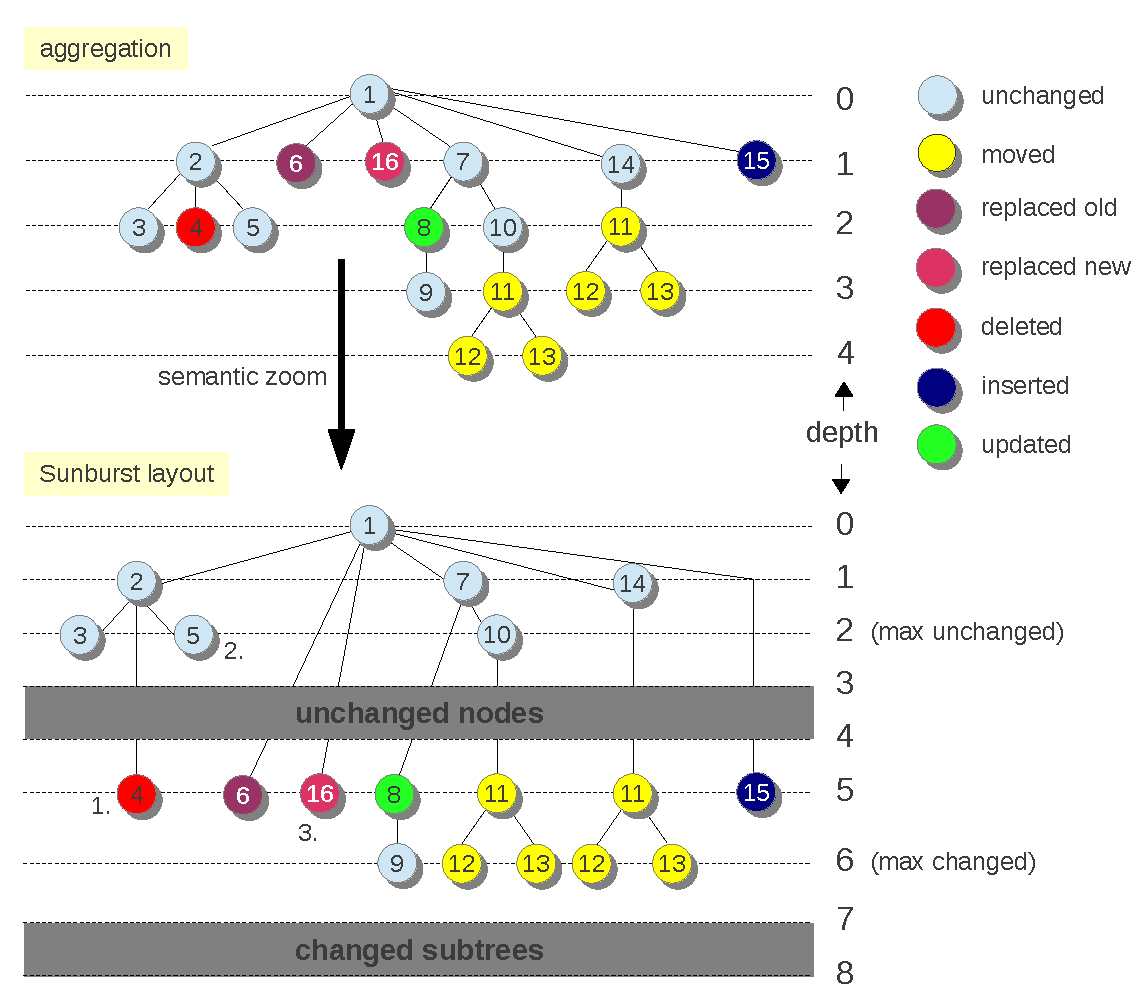
\includegraphics[width=\textwidth]
{figures/sunburst-layout}}
\caption{\label{fig:sunburst-layout} Sunburst-layout depicting changes in the depth. All nodes above the grey rectangle labeled ``unchanged nodes'' are unchanged whereas the area between the rectangle named ``changed subtrees'' and ``unchanged nodes'' includes all changed subtrees. However it also includes changed nodes below an updated node as for instance node 9.}
\end{figure}

Algorithm \ref{algo:calcDepth} determines if and how the depth must be adjusted. The first and second case is handled by the first \texttt{if}-clause, whereas the transition back to the original depth is handled by the \texttt{elseif}-clause. An instance variable \emph{mTempKey} is used to determine when to switch back. It is the node-ID of the first node in the XPath \texttt{following::}-axis. \emph{mTempKey} is adapted in case 3. such that it eventually contains the node-ID of an unchanged node. An \texttt{UPDATED} node most probably incorporates unchanged nodes if it is an internal \texttt{ElementNode}. In these cases the depth of the parent node plus one is used instead of the original depth such that the updated node \emph{and} its subtree are dislocated.

\begin{algorithm}[tb]
%\SetAlgoLined
\SetKwInOut{Input}{input}\SetKwInOut{Output}{output}
\Input{int pDepth, int pMaxDepth, DiffType pDiff, long mTempKey, long mInitDepth, int mPrunedNodes}
\Output{new depth}
\BlankLine
int depth $\leftarrow$ pDepth\;
\If{pDiff != DiffType.SAME AND pDiff != DiffType.SAMEHASH AND pDepth $\leq$ pMaxDepth + 2}{
  \tcp{Case 1 and 3.}
  depth $\leftarrow$ pMaxDepth + 2\;
  int index $\leftarrow$ mIndex + mPrunedNodes + mDescendantCount\;

  \If{index $<$ mDiffs.size()}{
    DiffTuple nextDiffTuple $\leftarrow$ mDiffs.get(index)\;
    DiffType nextDiff $\leftarrow$ nextDiffTuple.getDiff()\;
    boolean nextIsOldTransaction $\leftarrow$ isOldTransaction(nextDiff)\;

    mTempKey $\leftarrow$ 0\;
    \If{nextIsOldTransaction == true}{
      mTempKey $\leftarrow$ nextDiffTuple.getOldNodeKey()\;
    }\Else{
      mTempKey $\leftarrow$ nextDiffTuple.getNewNodeKey()\;
    }
  }
}\ElseIf{(pDiff == DiffType.SAME OR pDiff == DiffType.SAMEHASH) AND pDiffCont.getNewNodeKey() == mTempKey}{
  \tcp{Case 2.}
  depth $\leftarrow$ pDiffCont.getDepth().getNewDepth() - mInitDepth\;
}
\caption{Calculate depth}\label{algo:calcDepth}
\end{algorithm}

Besides adjusting the depth the semantic zoom requires some form of highlighting. In our case we opted for a global ``distortion'' which enlarges modified subtrees and shrinks subtrees of unchanged, potentially uninteresting nodes. Thus, the arc of a Sunburst item depends on two variables, the \texttt{subtree-size} and the number of \texttt{modification}s in a nodes' subtree.

\begin{equation}
ext = \left\{ \begin{array}{cl}
2 \cdot \pi & \textrm{if }node\ is\ root\ node\\
parExt \cdot ((1-\alpha) \cdot descs / (parDescs - 1) \\+ \alpha \cdot mods / (parMods - 1)) & \textrm{otherwise}\end{array}\right.
\end{equation}

The number of modifications in the forumla is derived from the \texttt{subtree-size} added to the number of \texttt{modification}s and multiplied by a constant. The addition of the \texttt{subtree-size} is needed to handle unchanged nodes, which do not contain any modifications in its subtree. In order to further emphasize and enlarge subtrees with a small number of modifications a constant is multiplied which has proven useful in empirical studies (Chapter \ref{sec::applications}). Furthermore note that if the parent node is modified the constant must be subtracted from the parent \texttt{modification}-count in advance.

The two variables are computed in parallel to the preorder traversal in the \texttt{Diff-Axis}. The results are appended to a thread safe queue designed for producer/consumer relationships. Modifications for the root node are gathered while observing diff-tuples, thus the number of modifcations does not need to be computed afterwards as for the other nodes in the agglomerated tree-structure. A simple heuristic determines depending on a depth-threshold if tasks are executed in the calling thread instead of another thread, as context switches for very small subtrees are too costly. Observe that the new descendant-count of each node in Treetank can not be used, because the aggregated tree-structure is traversed which incorporates deleted, replaced and moved nodes depending on settings (move- and replace-detection). Algorithm \ref{algo:descModCount} depicts how the two variables are derived by traversing the agglomeration at a specified index until the depth of a diff-tuple either is less than or equal to the start depth or no more diff-tuples are following thus forming a subtree-traversal. Note that the depth depends on the diff-type. In case of a \texttt{DELETED}, \texttt{MOVEDFROM} or \texttt{REPLACEDOLD} diff-type the depth of the node in the older revision is used, otherwise the depth of the node in the new revision. Furthermore recapitulate that the depths are computed by our ID-based diffing-algorithm instead of persistently stored as an attribute of the node by Treetank.

\begin{algorithm}[tb]
%\SetAlgoLined
\SetKwInOut{Input}{input}\SetKwInOut{Output}{output}
\Input{int pIndex, List pDiffs}
\Output{CONSTANT\_FACTOR * diffs, descendants, subtract}
\BlankLine
int index $\leftarrow$ pIndex\;
DiffTuple diffTuple $\leftarrow$ pDiffs.get(index)\;
DiffType diff $\leftarrow$ diffCont.getDiff()\;
int rootDepth $\leftarrow$ getDept(diff)\;

int diffs $\leftarrow$ 0\;
\If{diff != DiffType.SAME AND diff != DiffType.SAMEHASH}{
  diffs $\leftarrow$ 1\;
}
int descendants $\leftarrow$ 1\;
boolean subtract $\leftarrow$ false\;
index $\leftarrow$ index + 1\;

\If{diffCounts == 1 AND index $<$ pDiffs.size() AND hasFirstChild(pDiffs)}{
  \tcp{Current node is modified and has at least one child.}
  subtract $\leftarrow$ true\;
}

boolean done $\leftarrow$ false\;
\While{!done AND index $<$ pDiffs.size()}{
  diffTuple $\leftarrow$ pDiffs.get(index)\;
  diff $\leftarrow$ diffTuple.getDiff()\;
  int depth $\leftarrow$ getDept(diff)\;
  \If{depth $\leq$ rootDepth}{
    done $\leftarrow$ true\;
  }\Else{
    descendants $\leftarrow$ descendants + 1\;
    \If{currDiff != DiffKind.SAME AND currDiff != DiffKind.SAMEHASH}{
      diffs $\leftarrow$ diffs + 1\;
    }
    index $\leftarrow$ index + 1\;
  }
}
\caption{Computes the \texttt{subtree-size} of a node as well as the number of \texttt{modifications} in the nodes' subtree.}\label{algo:descModCount}
\end{algorithm}

\subsubsection{Filtering/Pruning}
Providing an initial Sunburst overview of huge tree-struc\-tures in reasonable time, ranging from a few seconds to a few minutes, requires pruning techniques to filter nodes of no or least interest. Therefore three types of filtering are provided. Changes in a nodes' subtree are always guaranteed to be visible. The following screenshots in this section are related to Fig. \ref{fig:without-pruning} which depicts the same tree comparison in the SunburstView without filtering nodes.

\begin{figure}[tb]
\center{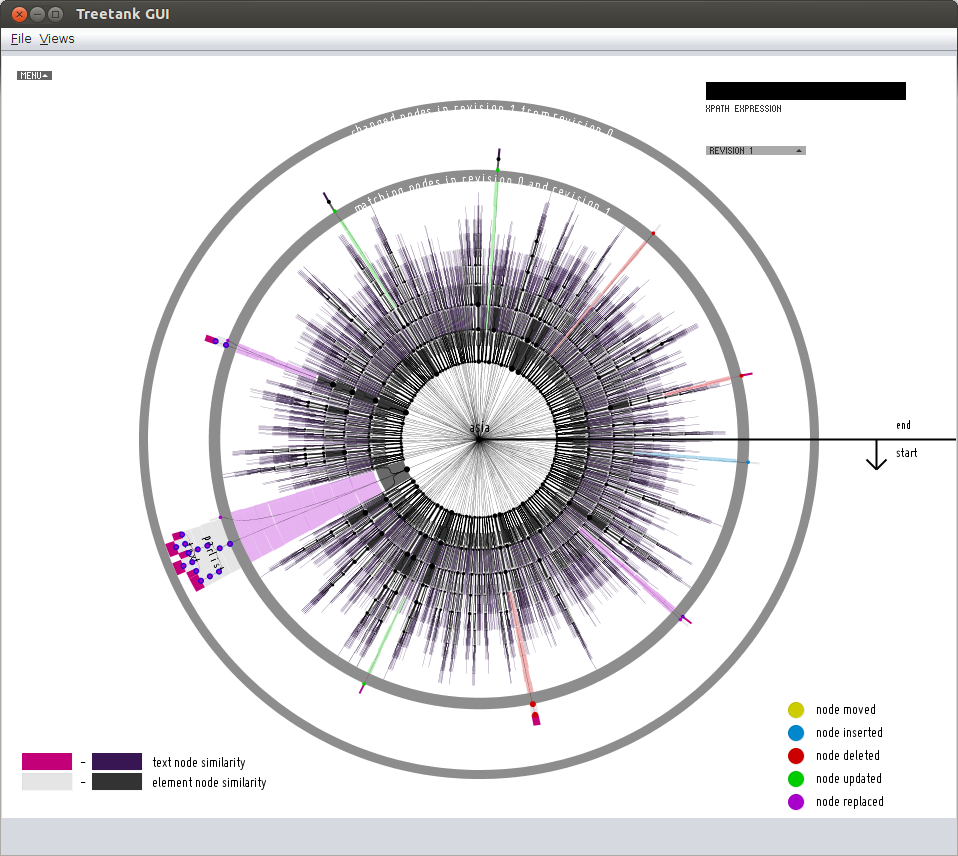
\includegraphics[width=\textwidth]
{figures/without-pruning}}
\caption{\label{fig:without-pruning} Comparison without pruning.}
\end{figure}

\begin{itemize}
\item \emph{by itemsize} Sunburst items which have no changes in its subtree and are too thin to be perceived individually or too thin to be selected even with the fisheye transformantion are pruned based on a predefined threshold-value. An example is depicted in Fig. \ref{fig:pruned-by-itemsize}. This type of filtering is useful wherever nodes which do not differ are of value but depicting the whole tree will not add any significant value. It considerably speeds up the generation of the Sunburst items in large tree-structures, however it does not affect the diff-calculation. Furthermore, if a new node is selected to drill down into the tree the items have to be rebuild, using the \texttt{Diff}-axis. Thus the optimization to create new items based on the initial set with adjusted angles is not usable. The \text{subtree-size} of each node as well as the number of \texttt{modifications} must be recalculated as well. 

\begin{figure}[tb]
\center{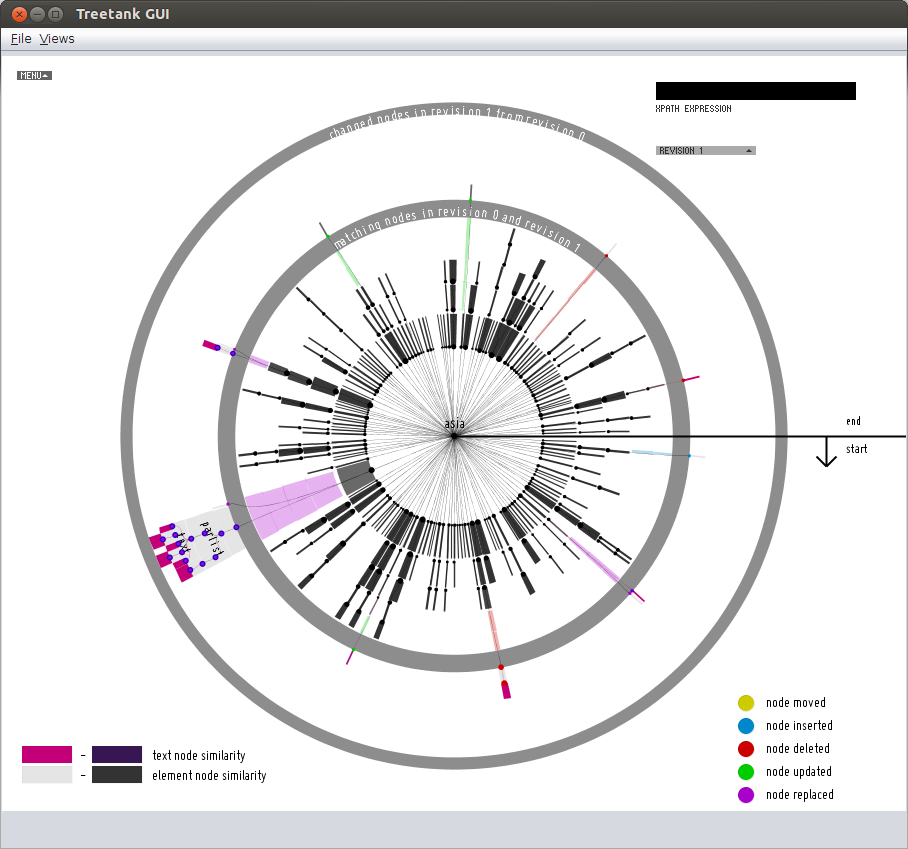
\includegraphics[width=\textwidth]
{figures/itemsize-pruned}}
\caption{\label{fig:pruned-by-itemsize} Pruned by itemsize.}
\end{figure}

\item \emph{by hash-based diff-algorithm} The diff-algorithm is invoked with the option to utilize persisted hashes which are created for every resource based on a database-configuration parameter. Per default a fast rolling-hash approach is used. All edit-operations thus only trigger a recomputation of the hashes of the ancestor-nodes based on the hash-value of the edited node. As described in Chapter \ref{sec::differences} everytime the hash values of the compared nodes are identical the traversal of both subtrees is skipped. Thus, items are only created for nodes, which include changed nodes in their subtree as well as for nodes with identical hash-values (Fig. \ref{fig:pruned-by-hash}). This type of pruning is especially useful for large tree-structures, whereas in contrast to the pruning by itemsize it speeds up the diff-computation as well as the item creation, as in both cases subtrees of nodes with identical hash-values are skipped. However, in comparison with the itemsize-based approach sometimes more items have to be created as nodes having identical hash-values are always included.

\begin{figure}[tb]
\center{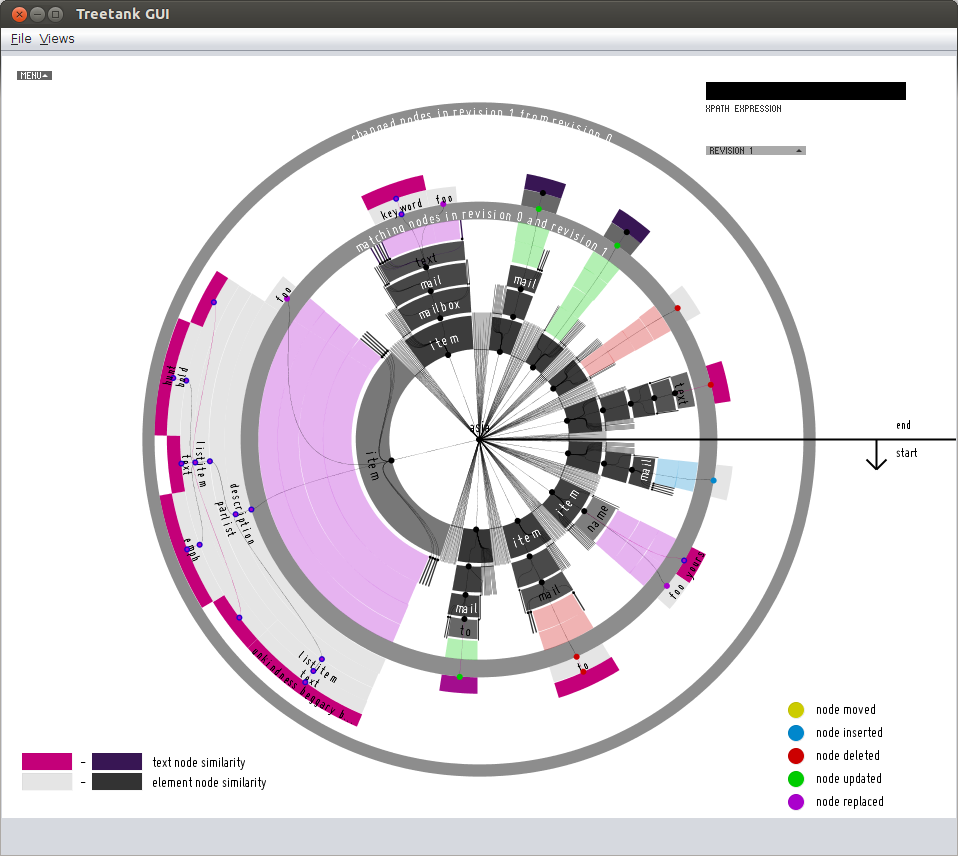
\includegraphics[width=\textwidth]
{figures/diff-pruned}}
\caption{\label{fig:pruned-by-hash} Pruned by identical hash-values.}
\end{figure}

\item \emph{by hash-based diff-algorithm without nodes which have the same hash} This type of pruning is related to the method described above. In addition to pruning nodes in the subtree of nodes with identical hash-values, additionally these subtree-roots are pruned, too. As a direct consequence the visualization is much better readability in case of many consecutive nodes with identical hash-values (Fig. \ref{fig:pruned-by-hash-without-samehashes}).

\begin{figure}[tb]
\center{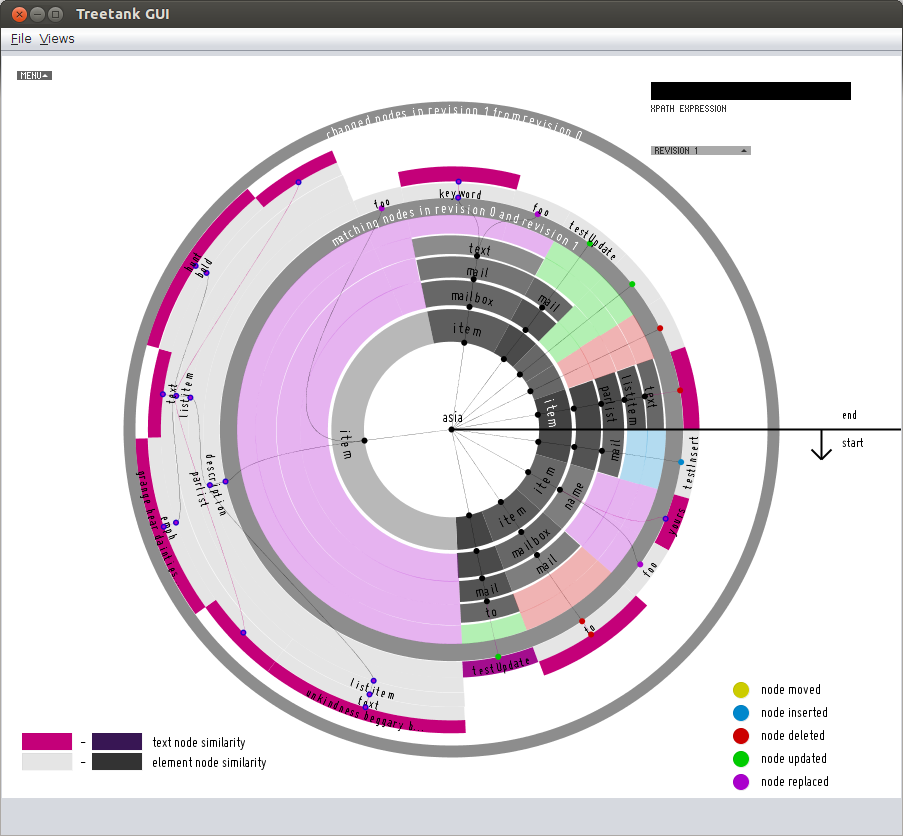
\includegraphics[width=\textwidth]
{figures/diff-without-samehashes-pruned}}
\caption{\label{fig:pruned-by-hash-without-samehashes} Pruned by identical hash-values without building items for nodes with identical hash-values.}
\end{figure}
\end{itemize}

Usually the maximum depth of unchanged nodes in the aggregated tree-structure is computed in a pipeline using a concurrent queue if more than two cores are available. Thus the computation is effectively parallelized with the diff-calculation. However, all above filtering types require postprocessing as maximum depth nodes might either be within the subtree of an unchanged node or in case of the itemsize-based filtering might be too thin regarding a threshold value und thus are pruned. Therefore, the maximum depth must be recomputed and the depth of changed nodes must be adapted accordingly. Note, that otherwise too much screen-space is wasted as the subtree-root of changed nodes is plotted between the maximum-depth of unchanged nodes plus two and the maximum depth plus three.

Having described several pruning-techniques and briefly meantioned a general zooming/panning technique based on affine transformations which is inherited from the \emph{SunburstView} layout depicting one revision the next section provides insight on how the selection of a new root-node to dig deeper into the tree-structure is handled. Note, that it is of the utmost importance to enlarge specific subtrees in the layout itself by user interaction. 

\subsubsection{Zooming / Details on demand} 
Supporting analysts with the ability to dig deeper into the tree-structure for most but the tiniest tree-structures is crucial. Thus we support the selection of a new root node through a mouse-click on the desired item. In our first prototype this triggered the recalculation of the diffs for the nodes' subtree as well as the maximum depth of unchanged nodes, the number of modifications and the subtree-size for each node in the subtree to build new enlarged items. Thus, a simple subtree-selection triggered the whole visualization-pipeline.

However due to unnecessary recalculations despite in case of the item-based pruning our optimized approach just recalculates the maximum depth of the unchanged nodes in parallel utilizing all available cores and subsequently builds new items based on angle-upscaling.

Having described the new Sunburst-layout tailored to comparison of tree-structures with all available pruning methods and the ability to select a new root-node in detail the next section describes how a similarity score between different types of nodes is measured, which is used for color-encoding of the items.

\subsubsection{Similarity measures}
Similarities for \texttt{Element}- and \texttt{Text}-nodes are measured differently. All non-leaf nodes of an XML-document are element nodes. However, if an element is a leaf node it is an \emph{empty element}.

\texttt{Element}-node similarity is measured based on overlapping subtrees. Consider the comparison of tree-structures T1 and T2. The similarity score for an element in the aggregated tree-structure $T_{aggr}$ is defined as

\begin{equation}
Sim(node_{T_{aggr}}) = \frac{descs(node_{T_{aggr}}) - mods(node_{T_{aggr}})}{descs(node_{T_{aggr}})}
\end{equation}

The similarity score is normalized between $[0, 1]$. The nodes of type\\ \texttt{INSERTED/DELETED/REPLACED} always are scored 0 as they do not have any equivalent in the other tree. In case of \texttt{SAME}-nodes the similarity depends on overlapping subtree-structures. If no modifications are in the subtree the score is 1. \texttt{UPDATED} nodes are modified and therefore add to the dissimilarity.

\texttt{Text}-nodes are leaf nodes which therefore have no child. We thus use a different similarity score defined as

\begin{equation}
Sim(node_{T_{aggr}}) = \left\{ \begin{array}{cl}
Levenshtein(node_{T_{1}}, node_{T_{2}}) & \textrm{if }node\ is\ \texttt{UPDATED}\\
0 & \textrm{if }node_{T_{aggr}}\ is \texttt{INSERTED}\\
  & \texttt{/DELETED/REPLACED}\\
1 & \textrm{otherwise}\end{array}\right.
\end{equation}

Note that the similarity score for updated nodes is computed based on the diff-tuple which incorporates both node-IDs. The Levenshtein algorithm is used, which defines a similarity score based on per-character edit-operations to change one string-value into the other one and is normalized between 0 (no similarity) and 1 (same string-value). 

In order to improve the usefulness of our visualizations we provide the ability to specify queries for specific nodes.

\subsection{Querying}
XPath 2.0 queries are currently partly supported by our XPath 2.0 engine. We also examined our Saxon\cite{Saxon} binding, which is surprisingly rather slow. However we did not measure time differences which is out of scope of this thesis. Future work most probabliy will include a Brackit\cite{Brackit} binding which is a ``flexible XQuery-based query engine'' developed at the TU Kaiserslautern. In contrast to Saxon it is specifically designed to work on top of databases and adding specific indexes for instance will be easy. However this feature is currently reevaluated.

We provide query capabilities on top of the agglomerated tree-structure and therefore query both compared revisions in parallel. The items are sorted by node-ID in parallel. Once all query results have been collected they are also sorted (the result is a sequence of node-IDs). A subsequent traversal of the items highlights query results.

\subsection{Visualization of moves}
Hierarchical Edge Bundles\cite{Bundles} avoid visual clutter of subtree moves. The technique creates a path up to but usually not including the Lowest Common Ancestor (LCA) of a source-node down to the destination-node. The path is used to define control points for plotting a curve.

The LCA is defined as:

\begin{equation}
lca(a{,} b) = min\{c|a \prec c, b \prec c\}
\end{equation}

A simple algorithm computes the LCA through adding elements on top of two stacks following the first node (moved from) and the second node (moved to) up to the root-node. In a next step the two stacks are processed in a loop removing the top element as long as identical node-IDs are found. The LCA is the last node-pair for which the node-IDs do match.

Fig. \ref{fig:moves} illustrates two move-operations on a subtree in a shakespear XML-document.

\begin{figure}[tb]
\center{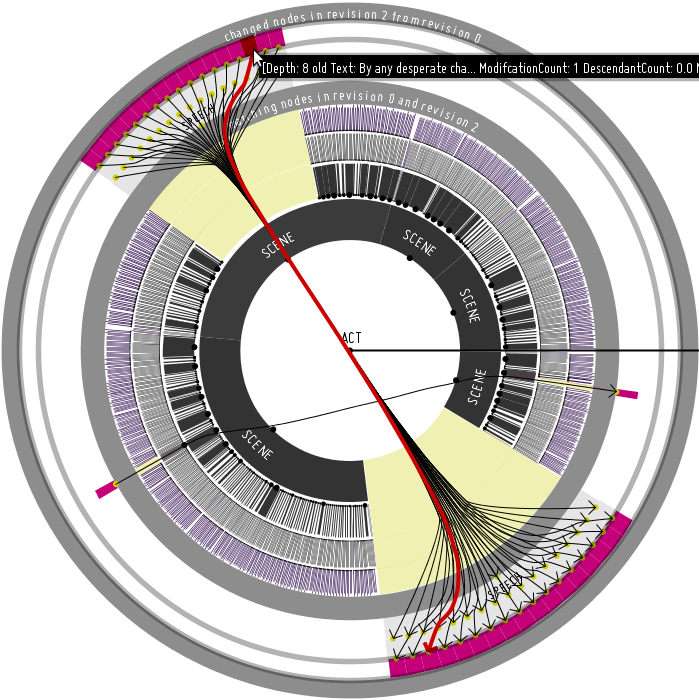
\includegraphics[width=\textwidth - 5em]
{figures/moves-cut}}
\caption{\label{fig:moves} Moves visualized using hierarchical edge bundles.}
\end{figure}

Despite comparing two tree-structures we furthermore aim to support a broad overview about the changes (and similarities) of multiple trees.

\subsection{Small multiple displays}\label{subsec::smallmultiple}
Small multiple displays of the \emph{SunburstView} provide an overview about the changes between several tree-structures. Two variants based on same-titled well known revisioning strategies as well as a hybrid variant are described next.

\begin{itemize}
\item \emph{differential} The differential variant displays changes related to a base revision. This is especially useful if several tree-structures have to be compared to a common base version. The direction is clockwise. That is the upper left corner displays a SunburstView comparison between revision 0 and 1 (if zero is the base revision which is loaded), the right upper corner displays changes between revision 0 and revision 2 et cetera (Fig. \ref{fig:smallmultiple-differential}).

\begin{figure}[tb]
\center{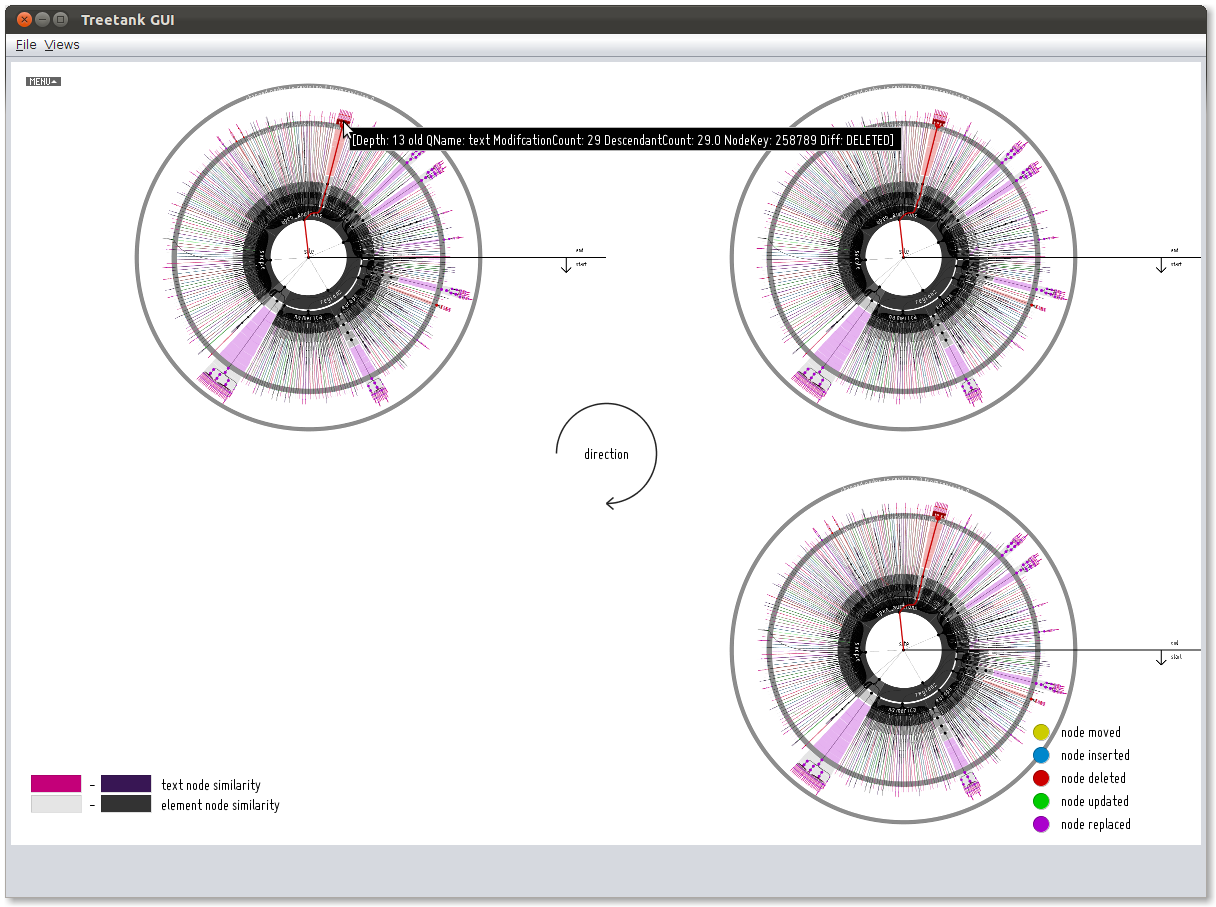
\includegraphics[width=\textwidth]
{figures/smallmultiple-differential}}
\caption{\label{fig:smallmultiple-differential} Small multiple - differential variant.}
\end{figure}

\item \emph{incremental} The incremental variant displays changes related to the last revision in increasing order. Suppose we have loaded revision 2, then in the upper left corner revision 2 and 3 is compared, the upper right corner contains the comparison between revision 3 and 4 et cetera (Fig. \ref{fig:smallmultiple-incremental}).

\begin{figure}[tb]
\center{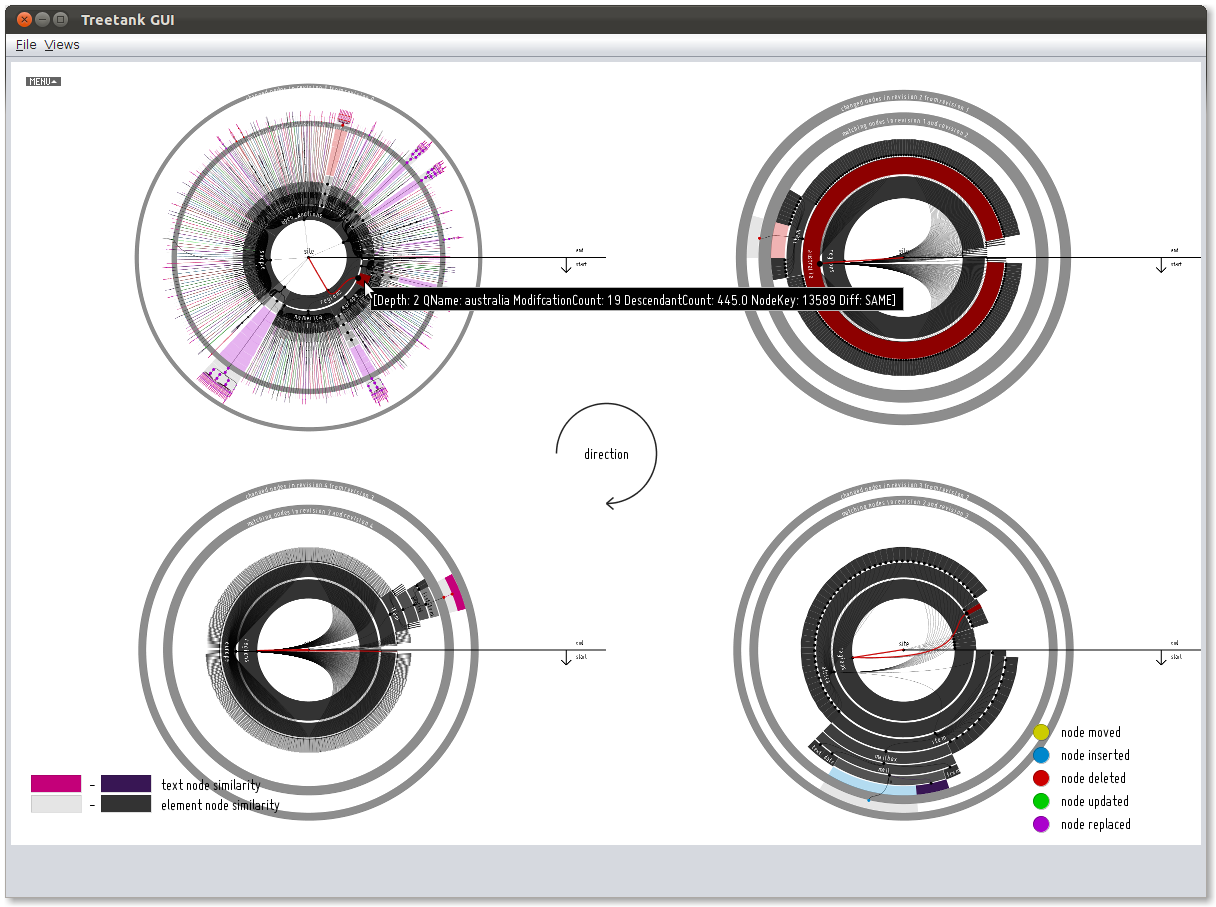
\includegraphics[width=\textwidth]
{figures/smallmultiple-incremental}}
\caption{\label{fig:smallmultiple-incremental} Small multiple - incremental variant.}
\end{figure}

\item \emph{hybrid} The hybrid variant displays changes just like in the incremental variant. However, a diff between the first revision and the last one to display is issued in the first place to get approximately the whole aggregated tree-structure. Upcoming changes in subsequent incremental comparisons are blackened. Furthermore, the colors denoting the changes lighten up in subsequent comparisons such that it is clear in which comparison the nodes are changed. During testing this view proved to be not as useful as we hoped. Nodes which are added in one revision and subsequently removed in another do not appear. In addition the colors denoting the type of change and during which comparison the change occured are too hard to distinguish in most cases.

\begin{figure}[tb]
\center{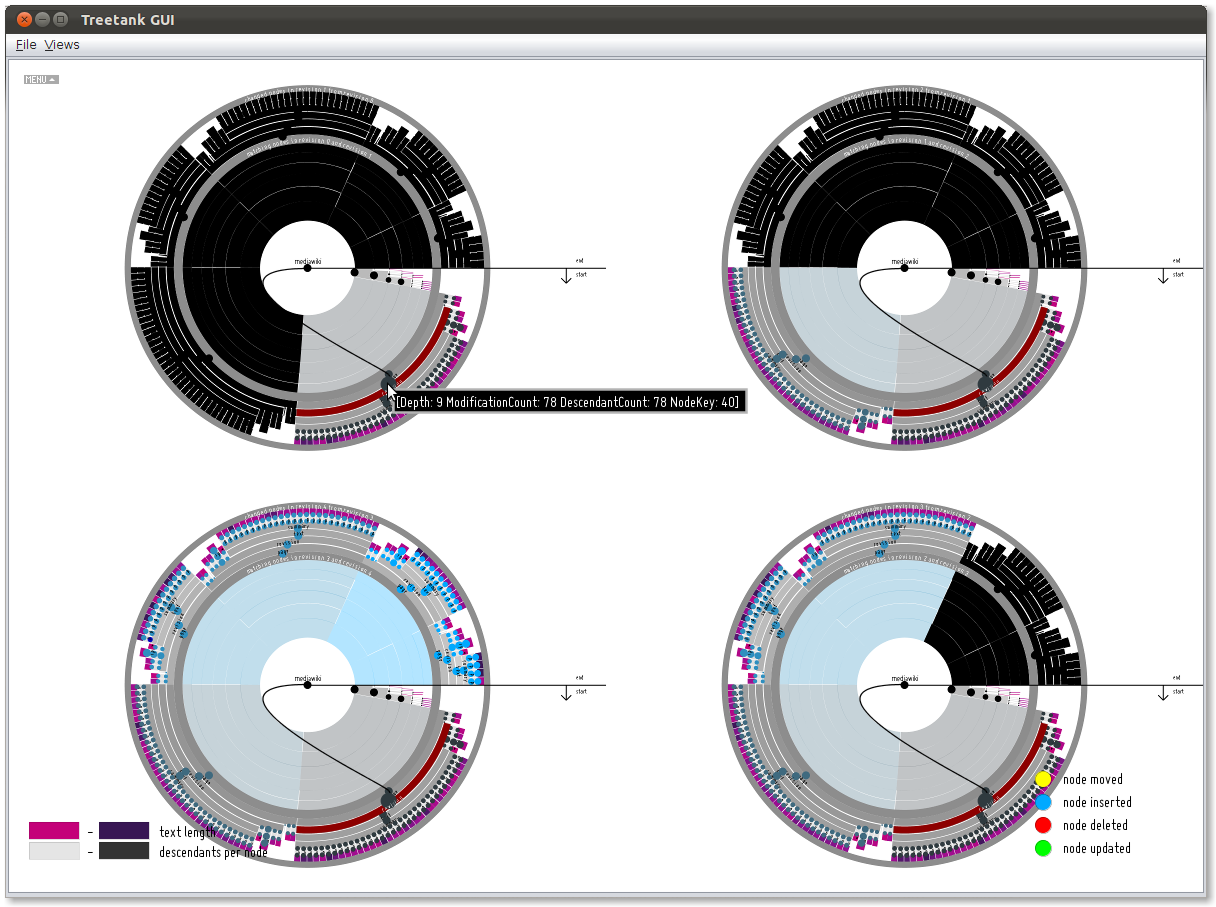
\includegraphics[width=\textwidth]
{figures/wikipedia-smallmultiples-hybrid}}
\caption{\label{fig:wikipedia-smallmultiples-hybrid} Small multiple - hybrid variant.}
\end{figure}
\end{itemize}

The implementation parallizes the computation of the small multiple displays and stores each Sunburst-visualization in an offscreen image, which is appended to a list in the view. This list must be sorted by revision-number after the items for all visualizations have been created. The more recent revision-number is saved along with the buffered offscreen image to support the clockwise order of comparisons. The items of each visualization are saved in a simple datastructure in the model to support highlighting of items on mouse over through brushing and linking. The technique is illustrated in Fig. \ref{fig:smallmultiple-differential} and \ref{fig:smallmultiple-incremental}. Items are highlighted in red just like in the SunburstView but the same item based on a node-ID equivalence relation is linked and highlighted in all small visualizations. Note that we aim to highlight whole subtrees on hovered nodes in a future version such that moves in the subtree during upcoming comparisons in the incremental variant will be easily visible resulting in forests. 

The two variants support all filtering methods described earlier. Next we provide a short asymptotic runtime- and space-analysis backed by performance measures.

\subsection{Runtime/Space analysis and scalability of the ID-based diff}
The runtime of the algorithm currently is bound by determining the subtree-size and modifications in the agglomerated tree-structure for each node. The runtime complexity thus is $O(n^2)$ whereas $n$ is the sum of changed and unchanged nodes between two trees $T1$ and $T2$. However by storing the diff-tuples which only include the depth of the two compared nodes to form a very simple tree-structure we are limited to a preorder traversal. Building a more sophisticated tree-structure based on pointers or sequences denoting child nodes for instance in an in-memory Treetank structure will support a subsequent postorder traversal to determine the subtree-size and modifications for each node reducing the runtime to $O(n)$. Due to using Java7 which is not available for OS X we are not able to measure the performance on computers with four or more cores. However, counting the subtree-size and modifications is started in parallel to building Sunburst items which consumes these through a Java \texttt{BlockingQueue}. Thus we assume adding more cores will speed up the creation of the items considerably as tree-structures often times are rather flat and have a large fan-out instead of being deep with high average levels/depths of the nodes, especially considering document-centric XML \cite{ronnau2009efficient}. The \texttt{subtree-size} of the root-item is the size of the accumulated List or Map of diff-tuples observed from the ID-based diffing algorithm and thus does not need to be computed. The number of \texttt{modifications} of the root-item is also determined on the fly while observing diff-tuples. Fig. \ref{fig:gui-performance} depicts performance measures, the average of ten runs of the Sunburst-visualization on an 11MiB-document and an 111MiB-document of the XMark-benchmark.  The documents are identical to the documents used in Chapter \ref{sec::differences} for benchmarking. Thus we randomly modified the instances after every 1000st node in the 11Mib-document and after every 10000st node in the 111MiB-document. The hardware used is also identical (Core 2 Duo 2666Mhz, 4Gb RAM). It is obvious that the exponential growth in case no pruning is enabled is unacceptable. Showing the 111MiB-document without pruning lasted too long (> 15min for each run) such that we aborted the execution. By reducing the number of Sunburst-items which have to be created considerably each one of the pruning-mechanisms reduces the runtime tremendously. Usually the number of Sunburst-items to create is reduced so much that the exponential time to compute the modifications in each nodes' subtree plus the subtree-size itself is not measurable and the runtime becomes linear. Furthermore as we are currently not able to measure the impact of parallelizing this task with four and more cores we can not measure the impact of parallelization which might also considerably speed up the computation without pruning. We assume that the context switches with only one or two cores in fact slow down the computation and thus introduced a simple threshold value to . 

Fig \ref{fig:gui-performance-movedet} shows benchmarking results comparing the runtime of the fastest pruning, pruning-by-hashes without creating items for identical hashes with move-detection enabled and disabled. We are able to determine that the move-detection usually is fast. Asymptotically it is bound by the size of the agglomerated tree-structure $n$, thus $O(n)$.

In summary we are able to conclude that the hash-based-pruning without creating Sunburst items is by far the fastest and that the move-detection usually does not inhibit the runtime of our algorithms considerably. Furthermore it is required to use pruning whenever the exponential time required to compute subtree-sizes and modifications therein significantly inreases due to a large aggregated tree. Adding more CPUs however should decrease the runtime as the computation of subtreesizes and modifications therein are computed in parallel.

\begin{figure}[tb]
\center{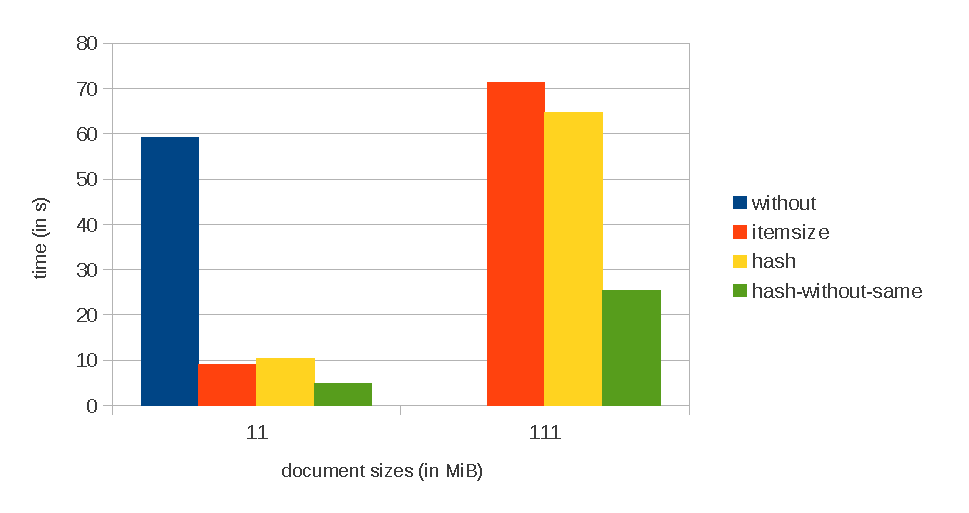
\includegraphics[width=\textwidth]
{figures/gui-performance}}
\caption{\label{fig:gui-performance} GUI-performance.}
\end{figure}

\begin{figure}[tb]
\center{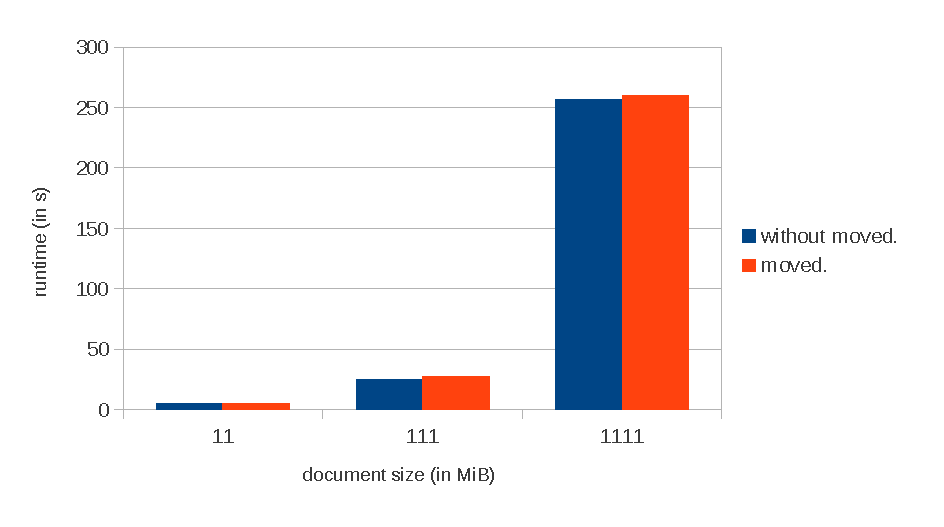
\includegraphics[width=\textwidth]
{figures/gui-performance-movedet}}
\caption{\label{fig:gui-performance-movedet} GUI-performance using hash-based pruning without adding identical hash-values and move-detection enabled/disabled.}
\end{figure}

\begin{table}[tb]
\centering 
\begin{tabular}[r]{|l|c|c|c|} 
\hline
& \textbf{1000mods} & \textbf{5000mods} & \textbf{10000mods}\\
\hline
\hline
\textbf{min} & 36265.14 & 35717.34 & 33948.96\\
\hline
\textbf{max} & 52459.38 & 61860.29 & 44451.06\\
\hline
\textbf{average} & 39167.75 & 37650.67 & 36579.37\\
\hline
\end{tabular}
\label{chap3:comparsion}
\vspace{0.5em} 
\caption{Comparsion of different modification-schemas of a 111 MiB XMark instance (change every 1000st, 5000st and 10000st node).}
\end{table}

\subsection{Conclusion and Summary}
We have introduced a multitude of visualizations ranging from a simple \emph{TextView} displaying syntax highlighted serialized XML in the viewport appending new text during scrolling to a \emph{SunburstView} and several \emph{Smallmultiple} display variants based on the \emph{SunburstView}. The \emph{TextView} supports the visualization of structural differences based on the aggregated tree structure and through a color-coded background depending on the diff-type. However non-structural changes, for instance the similarity between updated String values can not be visualized. Our main contribution is a new Sunburst layout based on the idea of a semantic zoom, which places all changed nodes prominently between two rings and facilitates a global distortion to enlarge changed-subtrees and thus to shrink unchanged subtrees accordingly which are potientially uninteresting. Structural changes are visualized through color coding of the node in the overlaying node-link diagram. The type of diff is indicated through a color-encoding. Furthermore the similarity of \texttt{TextNode} values and \texttt{ElementNode}s are depicted based on predefined functions. Large matched subtrees result in a higher similarity score for element nodes, few character replacements/inserts/deletes increases the similarity score for text nodes.

Moreover three filtering techniques facilitate the analysis of large tree-structures. Pruning by itemsize is useful if changed \emph{and} and unchanged nodes are of importance speeding up the creation of items considerably. However it does not affect the diff-computation. Thus, we also provide hash-based filtering techniques, which utilize the diff-algorithm with the optimization to skip the traversal of subtrees of nodes with identical hash-values. These filtering types usually reduce the number of items even more and accelerate the diff-computation. Note that the hashes include the unique node identifiers and other node-specific content, thus by using an exchangeable cryptographic hash-function th.  

Move-detection is enabled on demand. Furthermore inserted/deleted subtrees in a row are summarized as replace-operations.

In addition to the \emph{TextView} and \emph{SunburstView} small multiple variants support the comparison of multiple trees ($>2$). The number of comparsions is only limited by our implementation (which is only an implementation-detail) and the available screen space. Note, that the small multiple displays currently use too much unused screen space due to storing the whole visualization except the legends and menus in an offscreen image which are downscaled afterwards. As the extends of the main GUI-window usually are not squarified the space usually used for drawing menu-components and legends in the \emph{SunburstView} is multiplied and wasted. However this is merely an implementation detail which will be fixed in a future version. The filtering techniques are also available in the small multiple variants.
